% ============================================================================
% ArrowFlow v3 -- main manuscript (original article format)
% Preamble and macros: manuscript/manuscript_ArrowFlow_arxiv.tex, lines 1-36,
% copied unchanged. Sections are in sections/, figures in figures/, the
% bibliography in references_v3.bib. Build with ./build.sh; see style_sheet.md.
% ============================================================================
\documentclass[12pt]{article}
\usepackage{amsmath}
\usepackage{graphicx}
\usepackage{algorithm}
\usepackage{algpseudocode}
\usepackage[hidelinks]{hyperref}
\hypersetup{pdftitle={ArrowFlow: Training Ranking Filters with Position Votes},pdfauthor={Ozgur Yilmaz}}
% Long URLs may break after any digit or lowercase letter and stretch slightly, so the reference list has no loose
% lines; a line that cannot break within the tolerance (ArrowFlow is never hyphenated) may stretch a little more.
\makeatletter
\g@addto@macro{\UrlBreaks}{\do\0\do\1\do\2\do\3\do\4\do\5\do\6\do\7\do\8\do\9\do\a\do\b\do\c\do\d\do\e\do\f\do\g\do\h\do\i\do\j\do\k\do\l\do\m\do\n\do\o\do\p\do\q\do\r\do\s\do\t\do\u\do\v\do\w\do\x\do\y\do\z}
\makeatother
\setlength{\emergencystretch}{1.5em}
\Urlmuskip=0mu plus 1mu
\usepackage{natbib}
\usepackage{amsthm}
\usepackage{amssymb}
\usepackage{booktabs}
\usepackage{enumitem}
\usepackage{bm}
\usepackage{multirow}
\usepackage[section]{placeins}  % floats stay inside their own section
\usepackage[margin=1in]{geometry}
\usepackage{tikz}
\usepackage{pgfplots}
\pgfplotsset{compat=1.17}
\usetikzlibrary{arrows.meta, positioning, calc, patterns, decorations.pathreplacing, backgrounds, fit, shapes.geometric, matrix}

\DeclareTextSymbolDefault{\textbullet}{OMS}
\DeclareTextSymbolDefault{\textasteriskcentered}{OMS}
\hyphenation{ArrowFlow}
\newcommand{\R}{\mathbb{R}}
\newcommand{\Z}{\mathbb{Z}}
\newcommand{\E}{\mathbb{E}}
\newcommand{\norm}[1]{\left\lVert #1 \right\rVert}
\newcommand{\argsort}{\mathrm{argsort}}
\newcommand{\orderdesc}{\mathrm{argsort}_{\downarrow}}
\newcommand{\rankop}{\mathrm{rank}}
\newcommand{\softmax}{\mathrm{softmax}}

\newtheorem{theorem}{Theorem}
\newtheorem{lemma}[theorem]{Lemma}
\newtheorem{corollary}[theorem]{Corollary}
\newtheorem{proposition}[theorem]{Proposition}
\newtheorem{definition}[theorem]{Definition}
\newtheorem{remark}{Remark}

\begin{document}

\title{ArrowFlow: Training Ranking Filters\\with Position Votes}
\author{Ozgur Yilmaz\footnote{ozguryilmaz@atu.edu.tr; \url{https://scholar.google.com/citations?user=AIJWYCAAAAAJ}} \\
\small Department of Artificial Intelligence\\
\small Adana Science and Technology University, Adana, Turkey}
\date{}
\maketitle

% ============================================================================
% ABSTRACT
% ============================================================================
\begin{abstract}
ArrowFlow is a classifier whose layers work with rankings. Each layer holds learned rankings, the ranking filters, and outputs them sorted by footrule distance to its input. Training examples vote on where a filter's items should go. A weighted Borda count merges the votes, with no derivative computed. The position displacements (motions) returned by the output layer's votes train the hidden layers. A fixed encoder sorts projected features, and a nearest-neighbor vote reads the last hidden ranking. Under nested cross-validation on seventeen datasets, seven used during development and ten chosen by prespecified rules, training the ranking layers improves performance. Scrambled, the motions leave the network less accurate on most datasets than never moving its hidden filters. Turned into target scores, motions of the same kind also train a neural encoder network by gradient steps, without differentiating the sort. As a classifier, the trained encoder network is more accurate than the same network untrained on all 17, significantly on 11. Swapped into ArrowFlow, it raises mean accuracy on 11 datasets, significantly on one, and lowers it significantly on none. Training a neural network via discrete motion signals from a ranking layer is novel and one of the most important contributions of the paper. Counting the filter's current order as one more voter, the update rule violates independence of irrelevant alternatives by Arrow's theorem under a mild weight condition. So a filter's order of two items can change when a third moves.
\end{abstract}
\begin{quote}\small\noindent\textbf{Keywords:} ranking filters; permutation learning; Borda count; Arrow's impossibility theorem; Spearman's footrule; nearest-neighbor classification; alternatives to backpropagation; target propagation\end{quote}

% ============================================================================
% MAIN TEXT
% ============================================================================
% Supplement subsections typed below as "Section~S<n>.<m>"; build.sh checks each number against the built supplement.
% supplement-ref supp:iia=S1.1
% supplement-ref supp:borda=S1.8
% supplement-ref supp:learned-development=S6.2
\section{Introduction}\label{sec:intro}

Most neural networks store their inputs and their learned parameters as numbers, and they learn by following gradients. This paper asks whether a network can instead compute with rankings, ordered lists of items, and learn by counting votes. It also asks whether the signal of those votes can train an ordinary neural network as well. Codes built from orders appear in neuroscience and in similarity search (Section~\ref{sec:related}). Here the network learns the orders that it compares its inputs with.

ArrowFlow builds such a network from four ingredients:
\begin{itemize}[leftmargin=2em,topsep=2pt,itemsep=1pt]
  \item \textbf{Data points} are rankings. A ranking is a permutation of a fixed set of items, the vocabulary.
  \item \textbf{Learned filters} are rankings of the same vocabulary. Each \emph{ranking filter} is a permutation prototype, a learned ranking that an input is compared with.
  \item \textbf{Similarity} is Spearman's footrule distance. It counts the total number of positions by which the items of one ranking must move to match another \citep{diaconis1977footrule}.
  \item \textbf{Learning} reorders the items of a filter by counting votes for their positions. No derivative is computed.
\end{itemize}

An encoder turns a real-valued example into a ranking (Figure~\ref{fig:pipeline}). It expands, standardizes and projects the features, and then it sorts the projected scores. A \emph{ranking layer} holds a bank of ranking filters and outputs the bank in order of distance to its input, nearest filter first. That output is itself a ranking, so the next layer can read it. To predict, ArrowFlow compares an example's last hidden ranking with those of the training examples, and the nearest ones vote on the class. We call this step the nearest-neighbor readout. Several \emph{views}, each an encoder with its own trained network, then vote on the final class.

Training is the main contribution of this paper: a layer of ranking filters are adjusted based on motion signals that are coming from higher layers. It is similar to backpropagation, but it is on ranking filters. It is the first known method to train a hierarchical network through discrete signals that are not derivatives.
During training, the network gets one more layer, an output layer with one filter per class. When this layer assigns an example to the wrong class, the filter of the true class votes to move toward the example's last hidden ranking. The class filter and the example's ranking are both rankings of the same hidden filters. The signed differences between the positions that they give each hidden filter are called \emph{motions}, and the motions travel back down the network. If the class filter ranks a hidden filter earlier than the example's ranking does, that hidden filter votes to move toward its input. If the class filter ranks it later, the filter votes to move away. Nothing is differentiated along the way. Still, whenever the class filter votes, the motions are exactly half the gradient of the squared distance between the two rankings' positions, taken with respect to the positions of the hidden filters in the example's ranking. A hidden filter's vote then tends to move its position the way a gradient step would. So the vote stands in for the missing derivative of the sort, as a straight-through estimator does \citep{bengio2013estimating}. Such an estimator trains through a discrete step by replacing the step's derivative with a simple surrogate (Section~S1.8).

\begin{figure}[!htbp]
\centering
\resizebox{\textwidth}{!}{%
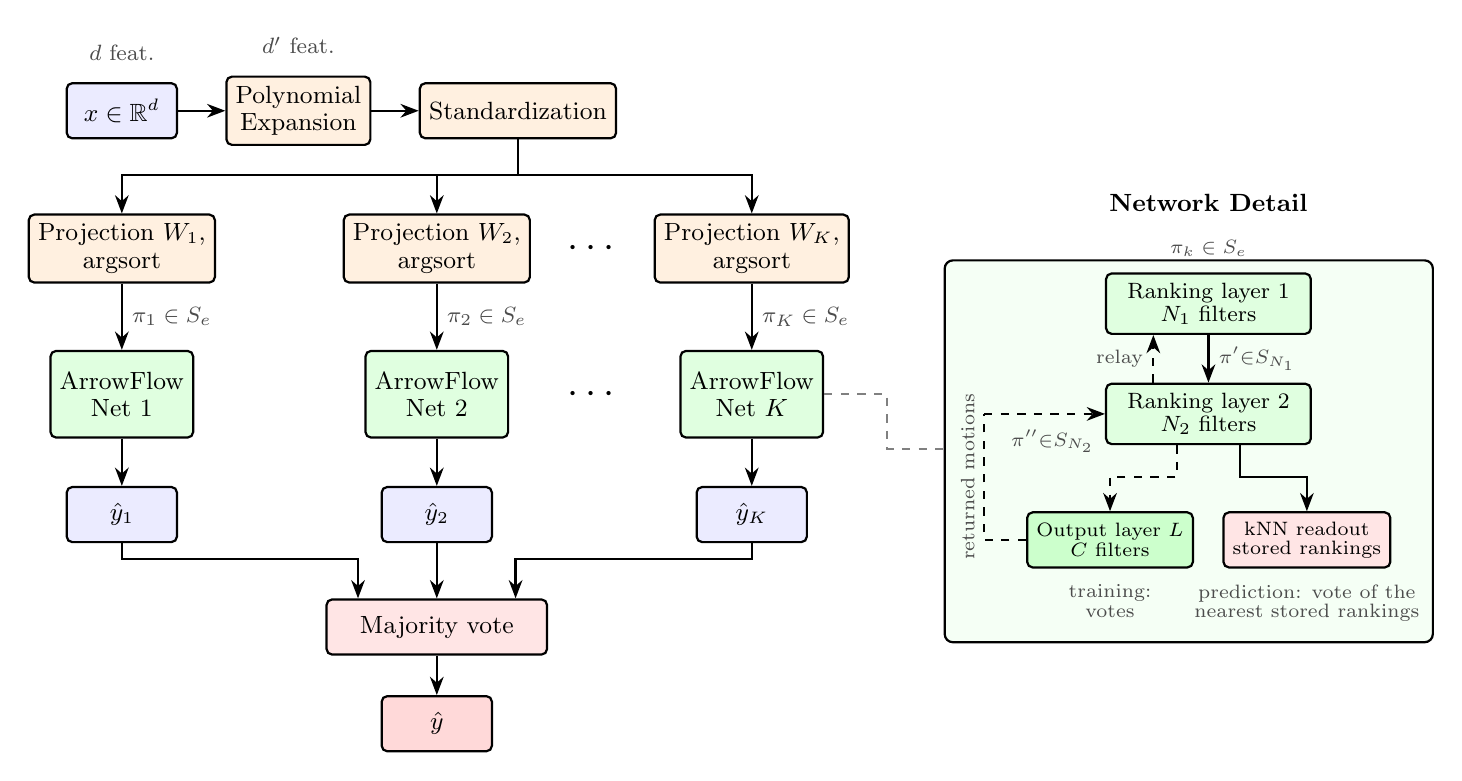
\begin{tikzpicture}[
    >=Stealth,
    box/.style={draw, rounded corners=2pt, minimum height=0.7cm, minimum width=1.4cm,
                font=\small, align=center, thick},
    databox/.style={box, fill=blue!8},
    procbox/.style={box, fill=orange!12},
    sortbox/.style={box, fill=green!12},
    votebox/.style={box, fill=red!10},
    arr/.style={->, thick},
    lbl/.style={font=\footnotesize, text=black!70},
]
% === Shared encoding steps (top row); every view expands and standardizes the same way ===
\node[databox] (input) at (0,0) {$x \in \R^d$};
\node[procbox, right=0.6 of input] (poly) {Polynomial\\[-1pt]Expansion};
\node[procbox, right=0.6 of poly] (std) {Standardization};
\draw[arr] (input) -- (poly);
\draw[arr] (poly) -- (std);
\node[lbl, above=0.15 of input] {$d$ feat.};
\node[lbl, above=0.15 of poly] {$d'$ feat.};
% === One projection and argsort per view: view k ranks the standardized features with its own W_k ===
\node[procbox] (proj1) at (0,-1.75) {Projection $W_1$,\\[-1pt]$\argsort$};
\node[procbox] (proj2) at (4,-1.75) {Projection $W_2$,\\[-1pt]$\argsort$};
\node[procbox] (projK) at (8,-1.75) {Projection $W_K$,\\[-1pt]$\argsort$};
\node at ($(proj2)!0.5!(projK)$) {\Large$\cdots$};
\draw[arr] (std.south) -- ++(0,-0.45) -| (proj1.north);
\draw[arr] (std.south) -- ++(0,-0.45) -| (proj2.north);
\draw[arr] (std.south) -- ++(0,-0.45) -| (projK.north);
% === Multi-view branching (3 networks), each reading its own input ranking ===
\node[sortbox, minimum height=1.1cm] (net1) at (0, -3.6) {ArrowFlow\\[-1pt]Net 1};
\node[sortbox, minimum height=1.1cm] (net2) at (4, -3.6) {ArrowFlow\\[-1pt]Net 2};
\node[sortbox, minimum height=1.1cm] (netK) at (8, -3.6) {ArrowFlow\\[-1pt]Net $K$};
\node at ($(net2)!0.5!(netK)$) {\Large$\cdots$};
\draw[arr] (proj1) -- node[lbl, right] {$\pi_1 \in S_e$} (net1);
\draw[arr] (proj2) -- node[lbl, right] {$\pi_2 \in S_e$} (net2);
\draw[arr] (projK) -- node[lbl, right] {$\pi_K \in S_e$} (netK);
% === Predictions ===
\node[databox, below=0.6 of net1] (pred1) {$\hat{y}_1$};
\node[databox, below=0.6 of net2] (pred2) {$\hat{y}_2$};
\node[databox, below=0.6 of netK] (predK) {$\hat{y}_K$};
\draw[arr] (net1) -- (pred1);
\draw[arr] (net2) -- (pred2);
\draw[arr] (netK) -- (predK);
% === Majority vote ===
\node[votebox, below=0.7 of pred2, minimum width=2.8cm] (vote) {Majority vote};
\draw[arr] (pred1.south) -- ++(0,-0.2) -| (vote.160);
\draw[arr] (pred2) -- (vote);
\draw[arr] (predK.south) -- ++(0,-0.2) -| (vote.20);
\node[databox, below=0.5 of vote, fill=red!15] (final) {$\hat{y}$};
\draw[arr] (vote) -- (final);
% === Network detail inset (far right, well separated) ===
\begin{scope}[shift={(13.8,-1.9)}]
\node[font=\small\bfseries, anchor=south] at (0,0.5) {Network Detail};
\draw[thick, rounded corners=3pt, fill=green!4] (-3.35,-4.85) rectangle (2.85,0);
\coordinate (insetleft) at (-3.35,-2.4);
\node[sortbox, minimum width=2.6cm, font=\footnotesize] (L1) at (0,-0.55) {Ranking layer 1\\[-1pt]$N_1$ filters};
\node[sortbox, minimum width=2.6cm, font=\footnotesize] (L2) at (0,-1.95) {Ranking layer 2\\[-1pt]$N_2$ filters};
\draw[arr] (L1) -- node[lbl, right, font=\scriptsize] {$\pi'{\in}S_{N_1}$} (L2);
\node[lbl, above=0.08 of L1, font=\scriptsize] {$\pi_k \in S_e$};
% below the last hidden layer: the output layer, used in training, and the nearest-neighbor readout, used to predict
\node[sortbox, minimum width=2.1cm, fill=green!20, font=\scriptsize] (Lout) at (-1.25,-3.55) {Output layer $L$\\[-1pt]$C$ filters};
\node[votebox, minimum width=2.1cm, font=\scriptsize] (RO) at (1.25,-3.55) {kNN readout\\[-1pt]stored rankings};
\draw[arr, dashed] ([xshift=-4mm]L2.south) -- ++(0,-0.4) -| (Lout.north);
\draw[arr] ([xshift=4mm]L2.south) -- ++(0,-0.4) -| (RO.north);
% training: the motions returned by the output votes train the last hidden layer (dashed, upward), which relays signed
% motions to the layer below (dashed, between the two hidden layers)
\draw[dashed, thick] (Lout.west) -- (-2.85,-3.55) -- (-2.85,-1.95);
\draw[arr, dashed] (-2.85,-1.95) -- (L2.west);
\node[lbl, font=\scriptsize, rotate=90, anchor=south] at (-2.85,-2.75) {returned motions};
\draw[arr, dashed] ([xshift=-7mm]L2.north) -- node[lbl, left, font=\scriptsize] {relay} ([xshift=-7mm]L1.south);
\node[lbl, font=\scriptsize, anchor=east] at (-1.33,-2.3) {$\pi''{\in}S_{N_2}$};
\node[lbl, below=0.08 of Lout, font=\scriptsize, align=center] {training:\\[-1pt]votes};
\node[lbl, below=0.08 of RO, font=\scriptsize, align=center] {prediction: vote of the\\[-1pt]nearest stored rankings};
\end{scope}
% Dashed connector from network box to inset
\draw[dashed, gray, thick] (netK.east) -- ++(0.8,0) |- (insetleft);
\end{tikzpicture}%
}
\caption{\textbf{ArrowFlow pipeline.} A real-valued input $x$ is encoded by polynomial expansion of degree $p$, standardization, a projection and argsort. The $K$ views use different projections $W_k$, $k = 1, \dots, K$, cycling through target-aware, random and calibrated strategies, so their networks receive different input rankings. Each network (detail, right) is a stack of ranking layers, and every layer ranks its ranking filters by Spearman's footrule distance to its input ranking. In training, an output layer holds one filter per class, and the filter of the example's class votes to move toward the last hidden ranking. The motions this vote returns train the last hidden layer, which relays signed motions to the preceding layer (dashed arrows). To predict, a nearest-neighbor (kNN) readout compares the last hidden ranking with the stored hidden rankings of the training examples. The $K$ predictions are combined by majority vote. $S_n$ denotes the set of rankings of $n$ items.}
\label{fig:pipeline}
\end{figure}


Every update of a ranking filter merges the rankings of a training batch into one, so every update is an election. Arrow's impossibility theorem \citep{arrow1951social,arrow1963social} says that no way of merging rankings has every property one might want. With three or more alternatives, no rule that turns every profile of rankings into one ranking satisfies three conditions at once: Pareto efficiency, independence of irrelevant alternatives and non-dictatorship. This is a lens to look at the update rule. It gives us a simple perspective on the context dependence of a filter's order of two items, which is essential for nonlinearity in the network.
Independence asks that the merged order of two items depend only on how the voters order those two items. Our update is a weighted Borda count, which orders items by their weighted sums of positions, and the filter's current order counts as one more voter. The rule is Pareto efficient for any positive weights. Under a mild condition on the weights it is also non-dictatorial, so it must break independence. The condition says that the votes of a batch weigh enough that they can move the filter. In ArrowFlow's layers, an update that holds the current order fixed is not Pareto efficient, so the theorem does not apply to it. It breaks independence too, by a direct construction, whenever its votes can move the filter (Section~S1.1). So a filter's order of two items can change when the training rankings move a third.

We use the theorem as a design lens, and it promises nothing about accuracy. It shows that this context dependence lives in the learning rule. And the voting reading names three stages of the network whose rules can be exchanged. The name joins \emph{Arrow}, for the vote inside every filter update, and \emph{Flow}, for the rankings that pass from layer to layer.

\paragraph{What this paper shows.} We did not build ArrowFlow to be the most accurate classifier, and it is not one. With all settings tuned on the training data alone, it trails the best tuned classical model on all seventeen tabular datasets we test (Table~\ref{tab:main}). Its average rank is fourth among the six tuned models, between random forest and gradient boosting, and fifth on the ten further datasets alone. What the paper shows instead is that votes, without computing any derivative, can train ranking layers, and that the motions they return can train an ordinary neural network:
\begin{enumerate}[leftmargin=2em,topsep=2pt,itemsep=1pt]
  \item \emph{Training helps.} The trained network is more accurate than an untrained ArrowFlow on 16 of the 17 datasets, although the untrained version comes within one percentage point on 12 of the 17 (Section~\ref{sec:training-controls}).
  \item \emph{The training signal carries information.} Suppose we scramble the motions but keep their sizes. The network then ends up less accurate than if its hidden filters had never moved. This happens on 16 of the 17 datasets when each motion reaches the wrong filter, and on 14 of the 17 when its direction is random. A post hoc test across the datasets, one defined after the results were known, supports both (Section~\ref{sec:motion-controls}).
  \item \emph{Motions also train a real-valued network.} Motions of the same kind can be turned into target values for the scores that a small encoder network sorts. They then train that network with a standard gradient-based optimizer, although the sort between the two is never differentiated. Other methods also train through an exact discrete step (Section~\ref{sec:related}). The trained encoder network is more accurate than the same network untrained on all 17 datasets, significantly on 11. Swapped into ArrowFlow for the fixed encoder, it raises the mean accuracy on 11 of the 17 datasets, significantly on balance-scale, and lowers it significantly on none (Section~\ref{sec:learned}). The conversion of motions into target scores and its settings were developed on single splits of twelve of the seventeen datasets (Section~S6.2).
  \item \emph{The contribution is the learning rule, and its limits are clear.} A support vector classifier with a fixed Kendall kernel, a standard similarity between rankings, is more accurate than ArrowFlow on 14 of the 17 datasets when both read rankings from the same encoder family. Read by that classifier, trained hidden rankings are no better than untrained ones. So training improves the neighborhoods of the nearest-neighbor readout, but the representation read by a strong fixed readout shows no gain. A second hidden layer did not help (Section~\ref{sec:controlled}).
\end{enumerate}
Sections~\ref{sec:related} to~\ref{sec:theory} cover related work, the network, the Arrow lens and the theory, and Section~\ref{sec:experiments} reports the experiments. Section~\ref{sec:discussion} discusses the results, and Section~\ref{sec:conclusion} concludes. The supplement, Sections~S1 to~S6, holds the proofs, the method details and protocol, the complete results, the ablations, the reproducibility records and the details of the trained encoder.

% Supplement subsections typed below as "Section~S<n>.<m>"; build.sh checks each number against the built supplement.
% supplement-ref supp:learning=S3.5
% supplement-ref supp:borda=S1.8
\section{Related Work}\label{sec:related}

ArrowFlow touches seven lines of work. The first studies ordinal codes and distances between rankings, and the second studies voting rules that combine rankings. The third covers prototype methods, and the fourth covers kernels, metric learning and symbolic vectors. The fifth covers alternatives to backpropagation, and the sixth covers ways to train through a sort. The seventh supplies the tools that ArrowFlow's pipeline borrows. For each line we say what it does and where ArrowFlow departs from it.

\paragraph{Ordinal codes and distances between rankings.}
The idea that order alone can carry information is old. Rank-order coding holds that the order in which neurons fire carries information about the stimulus \citep{thorpe1998rapid,gautrais1998rate,thorpe2001spike}, and \citet{bonilla2022analyzing} compare it with codes based on the time of the first spike. The rank transform of nonparametric statistics \citep{conover1981rank} also keeps only order. But it ranks one variable across observations, whereas top-scoring-pair classifiers compare pairs of features within one example \citep{geman2004classifying}. Rank-ordered autoencoders order hidden activations and learn sparse codes through progressive reconstruction \citep{bertens2016rank}. ArrowFlow instead feeds an ordinal code into layers of learned ranking filters and compares rankings by Spearman's footrule. \citet{diaconis1977footrule} show that the footrule stays within a factor of two of Kendall's distance, the number of item pairs that two rankings order differently \citep{kendall1938}. \citet{fagin2003topk} and \citet{fagin2006partial} extend both distances to top-$k$ lists and to partial rankings. Learning to rank \citep{burges2005learning,burges2010ranknet} fits a real-valued scoring function whose output is an ordering. In ArrowFlow, the inputs and the parameters are themselves orderings.

\paragraph{Voting rules and rank aggregation.}
Combining many rankings into one is the subject of social choice theory. Arrow's theorem \citep{arrow1951social,arrow1963social} limits every rule that turns a profile of rankings, one per voter, into one ranking. Positional rules, such as the Borda count \citep{young1974borda}, give each item points for its position on each ballot. Distance rules, such as the Kemeny median \citep{kemeny1959mathematics} and the footrule median, pick the ranking with the smallest total distance to the ballots. Both kinds have been compared in rank aggregation for metasearch \citep{dwork2001rank}. The Mallows model \citep{mallows1957nonnull} is a probability distribution over rankings that is centered on one modal ranking. \citet{conitzer2005voting} show which voting rules are maximum-likelihood estimators under which noise models, so choosing a rule also chooses what it estimates. Under Mallows noise, positional rules such as the Borda count recover the modal ranking as the number of votes grows \citep{caragiannis2013noisy}. The Borda count also combines the class rankings of several classifiers \citep{ho1994decision,vanerp2000variants}. ArrowFlow applies a weighted Borda count inside a learning system. Section~\ref{sec:arrow} states what Arrow's theorem implies for the network and what it does not.

\paragraph{Prototypes and reference objects.}
Many classifiers predict from distances to learned reference patterns. Learning vector quantization (LVQ) and self-organizing maps work this way \citep{kohonen1990self}, and so do generalized LVQ \citep{sato1995glvq,hammer2014learning,nebel2015median} and adaptive resonance theory \citep{grossberg1987competitive}. \citet{diao2021glvq} combine random-feature encodings with generalized LVQ and connect the result to hyperdimensional classifiers. ArrowFlow's output layer, which drives training, is a prototype classifier of this kind, with permutations as prototypes. Describing an object by its distances to reference objects is also the dissimilarity representation of \citet{pekalska2005dissimilarity}. Metric-space search goes one step further. It represents an object by the order of the reference objects by their distance to it, and it compares such orders with rank distances \citep{chavez2008proximity,amato2008approximate}. An untrained ranking layer read by a footrule nearest-neighbor vote is such a permutation index, with random rankings instead of data points as references. ArrowFlow learns the reference permutations and stacks the construction in layers. Random-weight networks fix random hidden units and train only a readout. Random vector functional-link networks \citep{pao1994learning} and extreme learning machines \citep{huang2006extreme,huang2012extreme} are examples, and random features approximate kernel machines in the same spirit \citep{rahimi2007random}. An untrained ArrowFlow is a permutation analog of these models.

\paragraph{Kernels, metric learning and symbolic vectors.}
Other methods also classify permutation-valued inputs, but they do not learn the permutations themselves. Kernels on permutations are the established supervised route. \citet{jiao2015kernels,jiao2018kendall} classify with Kendall and Mallows kernels, including numerical data converted to rankings, and they learn a decision function from pairwise similarities. Supervised metric learning fits a representation for a nearest-neighbor classifier \citep{goldberger2004nca,weinberger2009lmnn}. ArrowFlow instead trains its permutations against one prototype per class. Vector symbolic architectures and hyperdimensional computing (HDC) represent structured objects in high-dimensional distributed vectors. Holographic reduced representations bind and superpose vectors with circular convolution \citep{plate1995hrr}. Kanerva's construction labels an item's position before summation so that order survives \citep{kanerva2009hdc}, and ordered position codes serve biosignal classification \citep{rahimi2018biosignal}. The surveys of \citet{kleyko2022survey1,kleyko2023survey2} map the field. In these systems the state is distributed and algebraic. The codes are still related to ArrowFlow's. A thermometer code writes position $p$ as $p$ ones followed by zeros, and the footrule equals the Hamming distance between the thermometer codes of the positions. But ArrowFlow stores explicit permutations and updates them by position votes. Learned hyperdimensional classifiers train their class vectors \citep{duan2022lehdc,smets2025margin}, and \citet{verges2025hdcclassification} review and compare such classifiers. So the hyperdimensional control of Section~S3.5, an untrained classifier built from fixed random codes of items and positions, represents only its own construction. It says nothing about learned hyperdimensional classifiers. Discrete encoders can be trained with native integer and binary operations, with reported gains over untrained ones \citep{kirby2026encoder}.

\paragraph{Alternatives to backpropagation.}
The forward-forward algorithm \citep{hinton2022forward}, target propagation \citep{bengio2014auto} and its difference form \citep{lee2015difference}, and feedback alignment \citep{lillicrap2016random} avoid sending exact gradients back through a network, but they keep real-valued weights. ArrowFlow replaces the weights by permutations and updates them with position votes. Each batch update exactly minimizes a squared position objective of one filter (Section~S1.8), but no loss of the whole network is minimized. The output layer's vote only attracts the filter of the true class, whereas LVQ1 and LVQ2.1 also push a prototype of a wrong class away \citep{kohonen1990self}. A hidden layer computes the signal for the layer below from the permutations of its own selected filters. This is the analog of weight transport, the reuse of the forward weights to send errors back, which feedback alignment avoids. We do not propose the rule as a model of learning in the brain.

\paragraph{Training through a sort.}
Differentiable sorting replaces the permutation with a smooth approximation so that gradients can pass through it. NeuralSort \citep{grover2019neuralsort}, SoftSort \citep{prillo2020softsort}, projection onto the permutahedron \citep{blondel2020fast}, optimal transport \citep{cuturi2019ot} and Gumbel-Sinkhorn networks \citep{mena2018gumbelsinkhorn}, built on Sinkhorn normalization \citep{sinkhorn1967diagonal}, all work this way. ArrowFlow keeps the sort exact and never differentiates through it. Its trained encoder (Section~\ref{sec:learned-encoder}) also learns through an exact sort, by turning the motions into target scores in the spirit of target propagation \citep{bengio2014auto,lee2015difference}. Other methods also keep a discrete step exact. The straight-through estimator copies a gradient across the step as if the step were the identity \citep{bengio2013estimating,sahoo2023identity}. Blackbox differentiation interpolates the loss behind the solver, using a second call to the solver \citep{vlastelica2020differentiation,rolinek2020optimizing}. Perturbed optimizers average the solver's output over random perturbations of its input \citep{berthet2020perturbed}, and implicit maximum-likelihood estimation builds a target distribution for it \citep{niepert2021imle}. LambdaRank sets score gradients from desired rank changes \citep{burges2006nonsmooth}. The structured perceptron and its generalization, the Fenchel-Young losses, train a scoring model on the exact output of a solver \citep{collins2002perceptron,blondel2020fenchel}. Target propagation for hard-threshold units sets discrete targets for the hidden units and trains each unit toward them \citep{bengio2014auto,friesen2018combinatorial}. The trained encoder's targets come from motions toward a learned class filter and away from the nearest wrong one, and the example's own sorted scores turn them back into scores.

\paragraph{Random projections and ensembles.}
ArrowFlow's fixed encoder rests on random projection. The known guarantees on preserved distances \citep{johnson1984extensions,achlioptas2003database} and preserved margins \citep{arriaga2006algorithmic} concern the projected vector before sorting. The order of two Gaussian-projected coordinates is a random-hyperplane bit \citep{charikar2002similarity}, the sign of a random linear function of the input. The order of Gaussian projections also underlies the rank-order hashes for cosine similarity of \citet{eshghi2008locality}, and it relates to winner-take-all hashing \citep{yagnik2011power}. Section~\ref{sec:theory} states the resulting angle property. The multi-view ensemble is related to random-projection ensemble classification \citep{cannings2017random}, although ArrowFlow neither selects its projections nor thresholds the vote. It stands in the tradition of bagging \citep{breiman1996bagging}, boosting \citep{schapire1990strength}, ensemble diversity \citep{dietterich2000ensemble,kuncheva2003diversity} and multi-view learning \citep{xu2013survey}.

% Supplement subsections typed below as "Section~S<n>.<m>"; build.sh checks each number against the built supplement.
% supplement-ref supp:layer=S2.1
% supplement-ref supp:worked-example=S2.2
% supplement-ref supp:borda=S1.8
% supplement-ref tab:settings=S1
\section{The Ranking Layer}\label{sec:ranking-layer}

The ranking layer is the basic unit of ArrowFlow. It receives a ranking and measures how far that ranking lies from each ranking in a bank of learned rankings. Then it outputs the bank sorted by that distance. Learning reorders the learned rankings by collecting votes for where their items should sit, and no derivative is computed anywhere in the ranking layers. This section defines the layer, the training rule and the readout exactly.

\subsection{Notation}\label{sec:notation}

A \emph{ranking} of a vocabulary of $V$ items is a permutation $\pi$ that lists every item exactly once. We write $\pi[p]$ for the item at position $p\in\{1,\dots,V\}$ and $\operatorname{pos}_\pi(v)$ for the position of item $v$. The two maps are inverses, and $\operatorname{rev}(\pi)$ is $\pi$ read backwards. Worked examples list items by position, so $\pi=[C,A,E,B,D]$ means $\pi[1]=C$. Every item carries a distinct integer identifier (ID), and every sort in the method breaks exact ties by ascending ID (Section~S2.1). Table~\ref{tab:notation} collects the symbols used from here on.

\begin{table}[!htbp]
\caption{\textbf{Notation.} The layer superscript $(\ell)$ is dropped when a single layer is discussed.}
\label{tab:notation}
\centering
\small
\begin{tabular}{@{}l p{0.62\textwidth}@{}}
\toprule
Symbol & Meaning \\
\midrule
$\pi$, $\pi[p]$, $\operatorname{pos}_\pi(v)$, $\operatorname{rev}(\pi)$ & a ranking; its item at position $p$; the position of item $v$; the reversed ranking \\
$\pi_x$, $\pi'$ & the encoded input ranking; the output ranking of a layer \\
$V$ & vocabulary size of a layer, the number of items it ranks \\
$\ell$, $L$ & layer index and output layer; layer $\ell$ has vocabulary size $V_\ell$ and $N_\ell$ filters, and $V_{\ell+1}=N_\ell$ \\
$e$, $C$ & encoded vocabulary size, $V_1=e$; number of classes, $N_L=C$ \\
$r_j$, $N$ & ranking filter $j$ and the number of filters in a layer \\
$m_{\pi\to\tau}$, $m_j$ & motion of $\pi$ toward $\tau$, \eqref{eq:motion}; $m_j=m_{\pi_x\to r_j}$ \\
$\mathcal{M}^{(\ell)}$, $\mathcal{M}^{(\ell)}_j$ & signal list passed to layer $\ell$, sorted by $(-|\cdot|,\mathrm{ID})$; the entry of filter $j$ \\
$d_F$, $D_j$ & footrule distance, \eqref{eq:footrule}; $D_j=d_F(\pi_x,r_j)$ \\
$\pi^{(\ell)}$, $\hat y$ & output ranking of layer $\ell$, with $\pi^{(0)}=\pi_x$; class $\hat y=\pi^{(L)}[1]$ of the prototype readout \\
$A_j$, $A_j[p,k]$, $a$, $s_p$ & accumulator of filter $j$ (row $p$ is the item at position $p$, column $k$ a position); signed vote weight; mean voted position of row $p$ \\
$\eta$, $\rho$, $c$, $p_c$ & learning rate, selected fraction, signal scale, acceptance probability of a correct example \\
$w$, $g$ & sample weight (one throughout this paper); gate value in $\{0,1\}$ \\
$T$, $t$, $B$, $\nu$ & number of iterations, iteration index, batch size, validation fraction \\
$u$, $\tilde u$ & mean relayed motion and the scaled signal passed to the layer below, \eqref{eq:signal} \\
$h$, $\tilde h$, $q_p$, $m_y$, $m_w$ & for the encoder network of Section~\ref{sec:learned-encoder}: its scores, sorted in decreasing order into $\pi_x=\orderdesc(h)$; their targets; the target position of the coordinate at position $p$; the motions $m_j$ for $j=y$, the true class, and $j=w$, the nearest wrong class \\
\bottomrule
\end{tabular}
\end{table}

\subsection{Ranking Filters and Motions}\label{sec:filters}

A layer compares its input with each of its filters by asking how far the items must move. It holds $N$ \emph{ranking filters} $r_1,\dots,r_N$. A ranking filter is a permutation prototype, a learned permutation of the layer's vocabulary that the layer compares with its input.

The comparison rests on the \emph{motion} of one ranking $\pi$ toward another ranking $\tau$ of the same vocabulary,
\begin{equation}
m_{\pi\to\tau}[p]=\operatorname{pos}_\tau(\pi[p])-p,\qquad p=1,\dots,V,
\label{eq:motion}
\end{equation}
the signed number of positions that the item at position $p$ of $\pi$ must move to reach its position in $\tau$. A positive motion points toward the end of the ranking, and a negative one toward the front. For an input $\pi_x$ and a filter $r_j$ the motion is $m_j=m_{\pi_x\to r_j}$. Summing the absolute motions gives Spearman's footrule distance \citep{diaconis1977footrule},
\begin{equation}
d_F(\pi,\tau)=\sum_{p=1}^{V}\bigl|m_{\pi\to\tau}[p]\bigr|=\sum_{v}\bigl|\operatorname{pos}_\pi(v)-\operatorname{pos}_\tau(v)\bigr|.
\label{eq:footrule}
\end{equation}
The footrule is symmetric and takes even whole-number values from $0$ to $\lfloor V^2/2\rfloor$. It is the only distance the network computes, although the batch update minimizes squared position differences (Section~\ref{sec:theory-aggregation}). Figure~\ref{fig:forward-pass} shows the motions of one input toward three filters and the distances $D_j=d_F(\pi_x,r_j)$.

\begin{figure}[!htbp]
\centering
\resizebox{\textwidth}{!}{%
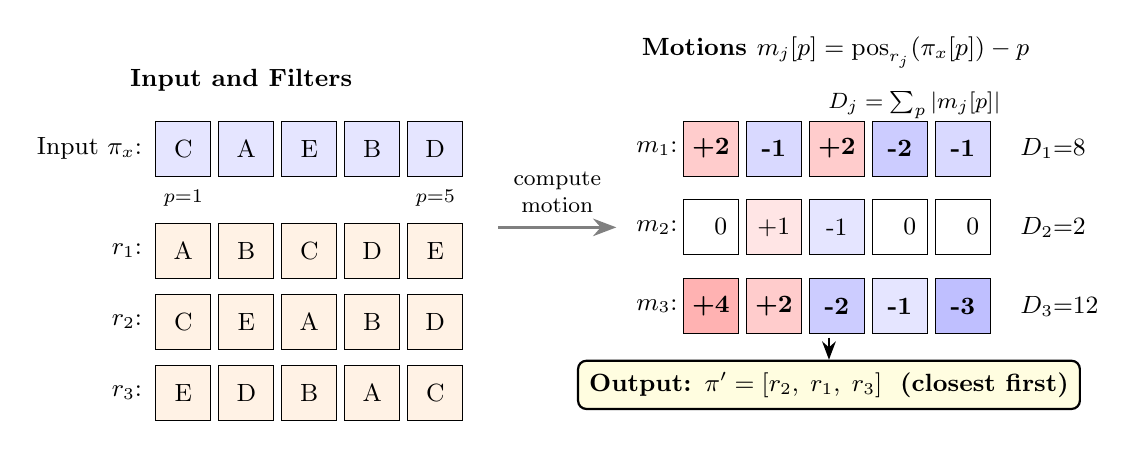
\begin{tikzpicture}[
    >=Stealth,
    arr/.style={->, thick},
    lbl/.style={font=\small},
    cell/.style={draw, minimum width=0.7cm, minimum height=0.7cm, font=\small, inner sep=0pt},
    hcell/.style={cell, fill=blue!10},
    fcell/.style={cell, fill=orange!10},
    mcell/.style={cell, fill=green!10},
]
% === LEFT HALF: Input + Filters ===
% Title
\node[font=\small\bfseries, anchor=south west] at (0.5, 1.8) {Input and Filters};
%
\node[lbl, anchor=east] at (0.9, 1.2) {Input $\pi_x$:};
\foreach \i/\v in {1/C, 2/A, 3/E, 4/B, 5/D} {
    \node[hcell] (in\i) at (0.5+\i*0.8, 1.2) {\v};
}
\node[lbl, below=0.04 of in1, font=\scriptsize] {$p{=}1$};
\node[lbl, below=0.04 of in5, font=\scriptsize] {$p{=}5$};
%
\node[lbl, anchor=east] at (0.9, -0.1) {$r_1$:};
\foreach \i/\v in {1/A, 2/B, 3/C, 4/D, 5/E} {
    \node[fcell] (f1\i) at (0.5+\i*0.8, -0.1) {\v};
}
\node[lbl, anchor=east] at (0.9, -1.0) {$r_2$:};
\foreach \i/\v in {1/C, 2/E, 3/A, 4/B, 5/D} {
    \node[fcell] (f2\i) at (0.5+\i*0.8, -1.0) {\v};
}
\node[lbl, anchor=east] at (0.9, -1.9) {$r_3$:};
\foreach \i/\v in {1/E, 2/D, 3/B, 4/A, 5/C} {
    \node[fcell] (f3\i) at (0.5+\i*0.8, -1.9) {\v};
}
% === Arrow between halves (above the rows, no overlap) ===
\draw[arr, gray, very thick] (5.3, 0.2) -- (6.8, 0.2);
\node[font=\footnotesize, black, above=2pt, align=center] at (6.05, 0.2) {compute\\motion};
% === RIGHT HALF: Motions ===
% Title
\node[font=\small\bfseries, anchor=south west] at (7.0, 2.1) {Motions $m_j[p] = \operatorname{pos}_{r_j}(\pi_x[p]) - p$};
%
\node[lbl, anchor=east] at (7.7, 1.2) {$m_1$:};
\foreach \i/\v/\c in {1/{+2}/red!20, 2/{-1}/blue!15, 3/{+2}/red!20, 4/{-2}/blue!20, 5/{-1}/blue!15} {
    \node[mcell, fill=\c, font=\small\bfseries] (m1\i) at (7.2+\i*0.8, 1.2) {\v};
}
\node[lbl, right=0.25 of m15] {$D_1{=}8$};
%
\node[lbl, anchor=east] at (7.7, 0.2) {$m_2$:};
\foreach \i/\v/\c in {1/{\phantom{+}0}/white, 2/{+1}/red!10, 3/{-1}/blue!10, 4/{\phantom{+}0}/white, 5/{\phantom{+}0}/white} {
    \node[mcell, fill=\c, font=\small] (m2\i) at (7.2+\i*0.8, 0.2) {\v};
}
\node[lbl, right=0.25 of m25] {$D_2{=}2$};
%
\node[lbl, anchor=east] at (7.7, -0.8) {$m_3$:};
\foreach \i/\v/\c in {1/{+4}/red!30, 2/{+2}/red!20, 3/{-2}/blue!20, 4/{-1}/blue!10, 5/{-3}/blue!25} {
    \node[mcell, fill=\c, font=\small\bfseries] (m3\i) at (7.2+\i*0.8, -0.8) {\v};
}
\node[lbl, right=0.25 of m35] {$D_3{=}12$};
% Formula note (below title, right-aligned)
\node[font=\footnotesize, anchor=east] at (11.8, 1.75) {$D_j = \sum_p |m_j[p]|$};
% === Output ranking ===
\node[draw, thick, rounded corners=3pt, fill=yellow!12, font=\small\bfseries, inner sep=4pt] (outbox) at (9.5,-1.8) {Output: $\pi' = [r_2,\; r_1,\; r_3]$ \;\small(closest first)};
\draw[arr, thick] (9.5, -1.2) -- (outbox.north);
\end{tikzpicture}%
}
\caption{\textbf{Ranking layer forward pass.} The input ranking $\pi_x = [C, A, E, B, D]$ is compared with three ranking filters $r_1, r_2, r_3$. The motion $m_j[p] = \operatorname{pos}_{r_j}(\pi_x[p]) - p$ is the signed displacement of the item at position $p$ toward its position in the filter (red: positive, toward the end of the ranking; blue: negative, toward the front). The footrule distance $D_j = \sum_p |m_j[p]|$ totals the displacements. The filters are ranked by distance, and $r_2$ (distance 2) is closest. The output ranking $\pi'$ is the input of the next layer.}
\label{fig:forward-pass}
\end{figure}


\subsection{Forward Pass}\label{sec:forward}

A layer's output is simply its filters, sorted from nearest to farthest, as in neural gas \citep{martinetz1993neural}. The output $\pi'$ lists the filter IDs sorted by $(D_j,j)$, closest first, with ties going to the lower ID. This output is a ranking of a new vocabulary, the $N$ filter IDs, and it is the next layer's input.

A network stacks $L$ ranking layers. Layer $\ell$ holds $N_\ell$ filters over $V_\ell$ items. The first layer ranks the $V_1=e$ items of the encoded input (Section~\ref{sec:encoding}), and every later layer ranks the filters of the layer below, so $V_{\ell+1}=N_\ell$. We write $\pi^{(0)}=\pi_x$ and $\pi^{(\ell)}$ for the output of layer $\ell$. The output layer $L$ holds $N_L=C$ filters, one per class, and its output $\pi^{(L)}$ is the \emph{class ranking}. The \emph{prototype readout} takes the class $\hat y=\pi^{(L)}[1]$, whose filter is nearest to the last hidden ranking $\pi^{(L-1)}$. The output layer only serves training. It drives the updates and makes none of ArrowFlow's predictions (Section~\ref{sec:prediction}, Table~\ref{tab:overview}).

% Method overview. Hand-written: it names parts and roles, not numbers.
\begin{table}[!htbp]
\caption{\textbf{What a view stores, and what each part is for.} A view is one encoder with the network trained on its rankings, and ArrowFlow trains $K$ of them (Section~\ref{sec:encoding}). A target-aware view puts coordinates fitted on the class labels before random ones, and a calibrated view standardizes its projected coordinates (Section~\ref{sec:encoder}). The output layer serves training and makes none of ArrowFlow's predictions.}
\label{tab:overview}
\centering
\footnotesize
\begin{tabular}{@{}p{0.19\textwidth} p{0.37\textwidth} p{0.34\textwidth}@{}}
\toprule
Part & What is fitted or stored & Role \\
\midrule
Encoder & imputation and standardization statistics and the projection matrix; a target-aware view also fits linear discriminant coordinates on the training labels, and a calibrated view stores the means and scales of its projected coordinates & turns a real-valued example into a ranking \\
\addlinespace
Hidden ranking layers & one permutation per ranking filter, reordered by position votes & produce the ranking that prediction reads \\
\addlinespace
Output layer & one permutation per class & gates the update, returns the signal from which every hidden layer learns, and scores the checkpoint \\
\addlinespace
Nearest-neighbor readout & the last hidden ranking of every training row with its label, and the chosen neighbor count and weighting & predicts the class of one view \\
\addlinespace
Vote across views & the predicted class of each view & gives the prediction of the ensemble \\
\bottomrule
\end{tabular}
\end{table}


\subsection{Position Votes and the Accumulator}\label{sec:accumulation}

Learning reorders a filter by counting votes for where each of its items should sit. Each filter $r_j$ owns an \emph{accumulator} $A_j\in\R^{V\times V}$, a table that collects these votes. Row $p$ belongs to the item $r_j[p]$ currently at position $p$, and column $k$ is a position. Between updates $A_j$ is the identity matrix, which gives every item one prior vote for its current position.

\begin{figure}[!htbp]
\centering
\resizebox{\textwidth}{!}{%
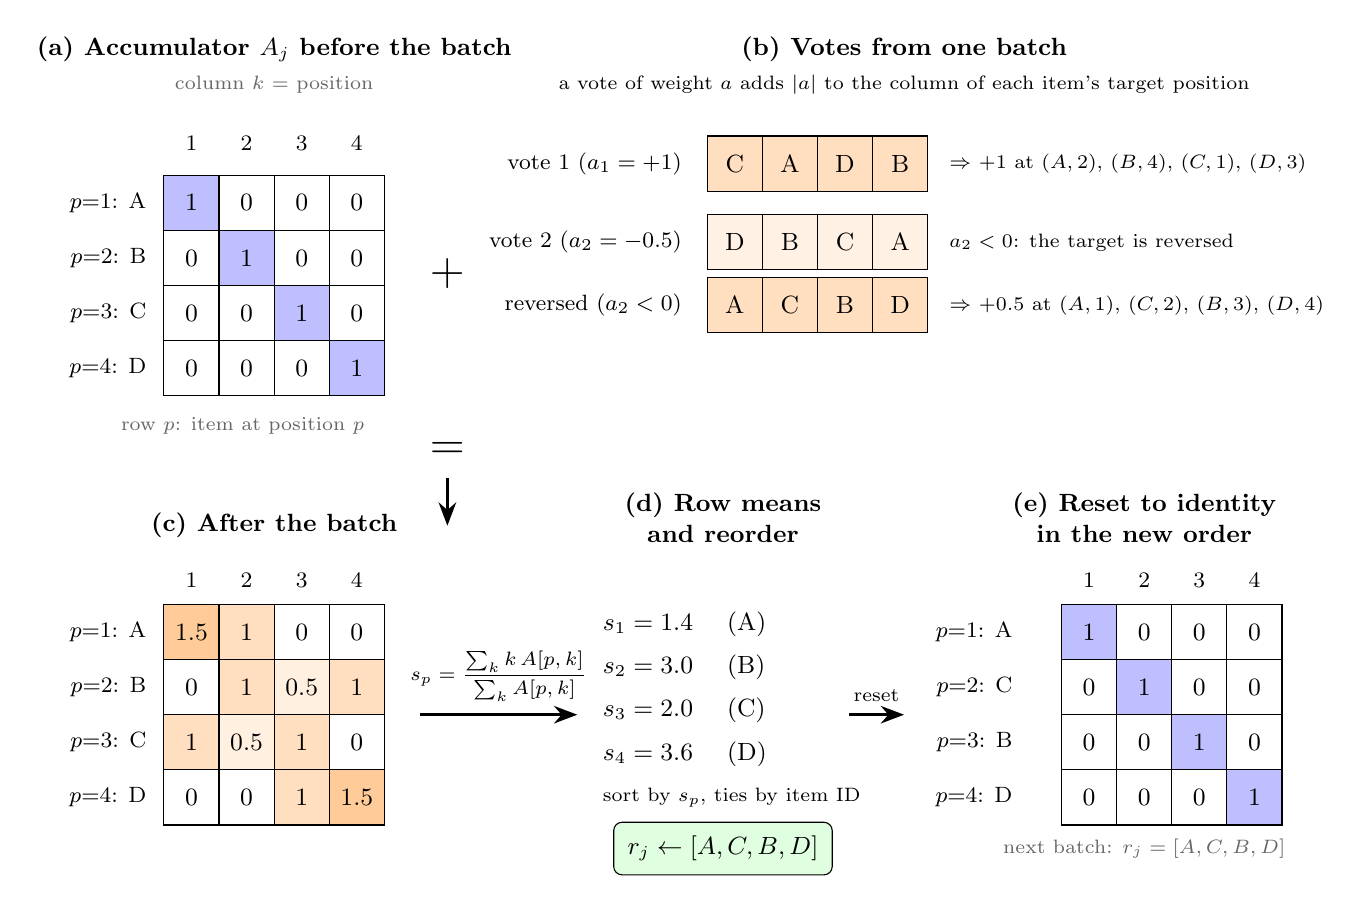
\begin{tikzpicture}[
    >=Stealth,
    arr/.style={->, thick},
    lbl/.style={font=\small},
    cell/.style={draw, minimum width=0.7cm, minimum height=0.7cm, font=\small, inner sep=0pt},
    tcell/.style={cell, fill=orange!25},
    rowlbl/.style={font=\footnotesize, anchor=east},
    colhdr/.style={font=\footnotesize},
    votelbl/.style={font=\footnotesize, anchor=east},
    note/.style={font=\scriptsize, text=black!60},
    ptitle/.style={font=\small\bfseries, align=center},
]
% ============================================================
% ROW 1:  (a) accumulator before the batch   +   (b) votes from one batch
% ============================================================
% --- (a) accumulator: identity in the current order r_j = [A,B,C,D] ---
\node[ptitle] at (1.4, 3.75) {(a) Accumulator $A_j$ before the batch};
\node[note] at (1.4, 3.3) {column $k$ = position};
\foreach \c in {1,2,3,4} {
    \node[colhdr] at (-0.35+\c*0.7, 2.55) {\c};
}
\foreach \r/\item in {1/A, 2/B, 3/C, 4/D} {
    \node[rowlbl] at (-0.1, 2.5-\r*0.7) {$p{=}\r$: \item};
    \foreach \c in {1,2,3,4} {
        \pgfmathtruncatemacro{\val}{\r==\c ? 1 : 0}
        \pgfmathtruncatemacro{\shade}{\r==\c ? 25 : 0}
        \node[cell, fill=blue!\shade] at (-0.35+\c*0.7, 2.5-\r*0.7) {\val};
    }
}
\node[note, anchor=north] at (1.0, -0.8) {row $p$: item at position $p$};
% --- plus sign ---
\node[font=\LARGE\bfseries] at (3.6, 0.9) {$+$};
% --- (b) votes from one batch ---
\node[ptitle] at (9.4, 3.75) {(b) Votes from one batch};
\node[note, text=black] at (9.4, 3.3) {a vote of weight $a$ adds $|a|$ to the column of each item's target position};
% vote 1: positive weight
\node[votelbl] at (6.7, 2.3) {vote 1 ($a_1 = {+}1$)};
\foreach \i/\v in {1/C, 2/A, 3/D, 4/B} {
    \node[tcell] at (6.55+\i*0.7, 2.3) {\v};
}
\node[font=\scriptsize, anchor=west] at (9.85, 2.3) {$\Rightarrow$ ${+}1$ at $(A,2)$, $(B,4)$, $(C,1)$, $(D,3)$};
% vote 2: negative weight, target reversed
\node[votelbl] at (6.7, 1.3) {vote 2 ($a_2 = {-}0.5$)};
\foreach \i/\v in {1/D, 2/B, 3/C, 4/A} {
    \node[tcell, fill=orange!10] at (6.55+\i*0.7, 1.3) {\v};
}
\node[font=\scriptsize, anchor=west] at (9.85, 1.3) {$a_2 < 0$: the target is reversed};
\node[votelbl] at (6.7, 0.5) {reversed ($a_2 < 0$)};
\foreach \i/\v in {1/A, 2/C, 3/B, 4/D} {
    \node[tcell] at (6.55+\i*0.7, 0.5) {\v};
}
\node[font=\scriptsize, anchor=west] at (9.85, 0.5) {$\Rightarrow$ ${+}0.5$ at $(A,1)$, $(C,2)$, $(B,3)$, $(D,4)$};
% ============================================================
% Equals sign + down arrow
% ============================================================
\node[font=\LARGE\bfseries] at (3.6, -1.35) {$=$};
\draw[arr, very thick] (3.6, -1.7) -- (3.6, -2.3);
% ============================================================
% ROW 2:  (c) after the batch  ->  (d) row means and reorder  ->  (e) reset
% ============================================================
% --- (c) accumulator after the batch (identity prior + both votes) ---
\node[ptitle] at (1.4, -2.3) {(c) After the batch};
\foreach \c in {1,2,3,4} {
    \node[colhdr] at (-0.35+\c*0.7, -3.0) {\c};
}
\node[rowlbl] at (-0.1, -3.65) {$p{=}1$: A};
\node[cell, fill=orange!40] at (0.35, -3.65) {1.5};
\node[cell, fill=orange!25] at (1.05, -3.65) {1};
\node[cell] at (1.75, -3.65) {0};
\node[cell] at (2.45, -3.65) {0};
%
\node[rowlbl] at (-0.1, -4.35) {$p{=}2$: B};
\node[cell] at (0.35, -4.35) {0};
\node[cell, fill=orange!25] at (1.05, -4.35) {1};
\node[cell, fill=orange!12] at (1.75, -4.35) {0.5};
\node[cell, fill=orange!25] at (2.45, -4.35) {1};
%
\node[rowlbl] at (-0.1, -5.05) {$p{=}3$: C};
\node[cell, fill=orange!25] at (0.35, -5.05) {1};
\node[cell, fill=orange!12] at (1.05, -5.05) {0.5};
\node[cell, fill=orange!25] at (1.75, -5.05) {1};
\node[cell] at (2.45, -5.05) {0};
%
\node[rowlbl] at (-0.1, -5.75) {$p{=}4$: D};
\node[cell] at (0.35, -5.75) {0};
\node[cell] at (1.05, -5.75) {0};
\node[cell, fill=orange!25] at (1.75, -5.75) {1};
\node[cell, fill=orange!40] at (2.45, -5.75) {1.5};
% --- arrow (c) -> (d) with the row-mean formula ---
\draw[arr, very thick] (3.25, -4.7) -- node[above=1pt, font=\scriptsize] {$s_p = \dfrac{\sum_k k\,A[p,k]}{\sum_k A[p,k]}$} (5.25, -4.7);
% --- (d) row means and reorder ---
\node[ptitle] at (7.1, -2.2) {(d) Row means\\and reorder};
\node[lbl, anchor=west] at (5.45, -3.55) {$s_1 = 1.4$ \quad (A)};
\node[lbl, anchor=west] at (5.45, -4.1) {$s_2 = 3.0$ \quad (B)};
\node[lbl, anchor=west] at (5.45, -4.65) {$s_3 = 2.0$ \quad (C)};
\node[lbl, anchor=west] at (5.45, -5.2) {$s_4 = 3.6$ \quad (D)};
\node[font=\scriptsize, anchor=west] at (5.45, -5.75) {sort by $s_p$, ties by item ID};
\node[draw, rounded corners=3pt, fill=green!12, font=\small, inner sep=5pt] at (7.1, -6.4) {$r_j \leftarrow [A, C, B, D]$};
% --- arrow (d) -> (e) ---
\draw[arr, very thick] (8.7, -4.7) -- node[above=1pt, font=\scriptsize] {reset} (9.4, -4.7);
% --- (e) reset to identity in the new order ---
\node[ptitle] at (12.45, -2.2) {(e) Reset to identity\\in the new order};
\foreach \c in {1,2,3,4} {
    \node[colhdr] at (11.05+\c*0.7, -3.0) {\c};
}
\foreach \r/\item in {1/A, 2/C, 3/B, 4/D} {
    \node[rowlbl] at (10.9, -2.95-\r*0.7) {$p{=}\r$: \item};
    \foreach \c in {1,2,3,4} {
        \pgfmathtruncatemacro{\val}{\r==\c ? 1 : 0}
        \pgfmathtruncatemacro{\shade}{\r==\c ? 25 : 0}
        \node[cell, fill=blue!\shade] at (11.05+\c*0.7, -2.95-\r*0.7) {\val};
    }
}
\node[note, anchor=north] at (12.45, -6.15) {next batch: $r_j = [A,C,B,D]$};
\end{tikzpicture}%
}
\caption{\textbf{Accumulation and reorder of one ranking filter.} (a)~The accumulator $A_j$ of the filter $r_j = [A,B,C,D]$ starts as the identity in the current order: row $p$ belongs to the item at position $p$ and column $k$ is a position. (b)~Two votes from one batch. A vote of weight $a$ toward a target ranking adds $|a|$ to the column of each item's position in the target~\eqref{eq:vote}; a negative weight reverses the target first. (c)~The accumulator after the batch. (d)~The mean voted position $s_p$ of every row~\eqref{eq:rowmean}. Sorting the items by $s_p$, with ties broken by item ID, gives the new filter $[A,C,B,D]$. (e)~The accumulator is reset to the identity in the new order before the next batch.}
\label{fig:accumulation}
\end{figure}


A training example casts position votes with a signed weight $a$ toward a target ranking $\tau$. A positive vote pulls the filter toward $\tau$. A negative vote pulls it toward the reversal of $\tau$, which acts as a push away. The target actually used is therefore $\tilde\tau=\tau$ when $a>0$ and $\tilde\tau=\operatorname{rev}(\tau)$ when $a<0$, and every item of the filter votes for its position in $\tilde\tau$:
\begin{equation}
A_j\bigl[p,\operatorname{pos}_{\tilde\tau}(r_j[p])\bigr]\leftarrow A_j\bigl[p,\operatorname{pos}_{\tilde\tau}(r_j[p])\bigr]+|a|,\qquad p=1,\dots,V.
\label{eq:vote}
\end{equation}
A zero weight adds nothing. The vote also returns $\operatorname{sign}(a)\,m_{r_j\to\tau}$, the motion of the filter toward the unreversed target, negated when the vote pushes away. The training procedure passes this motion to the layer below.

After all the votes of a batch are in, each row's mean voted position
\begin{equation}
s_p=\frac{\sum_{k=1}^{V}k\,A_j[p,k]}{\sum_{k=1}^{V}A_j[p,k]},
\label{eq:rowmean}
\end{equation}
reorders the filter. The items $r_j[p]$ are sorted by $(s_p,\mathrm{ID})$, with the row means compared as computed (Table~S1). A filter that receives no votes keeps its order. Then $A_j$ is reset to the identity in the new order. So the accumulator keeps no evidence from one batch to the next, and only the updated filter orders carry earlier training forward. Figure~\ref{fig:accumulation} traces one update. Ranking items by their mean voted position is a Borda count, a voting rule that scores each item by the positions it receives. Section~\ref{sec:arrow} develops this reading.

% No \FloatBarrier here: while Figure 3 was still waiting for its float page, the barrier forced a page break after the
% last three lines of this subsection and left a nearly empty page. Without it, Figure 3 still prints between the start
% of Section 3.4 and the start of Section 3.5; recheck that placement after any edit that moves text in this section.
\subsection{Supervised Training}\label{sec:training}

Training turns classification errors into votes, layer by layer from the top. Each iteration draws a batch and runs the forward pass with the filters held fixed. Then it updates the layers from the output layer down. In outline, every misclassified example votes to move the filter of its class toward the ranking that the example presents to the output layer, and so does a small random share of the correctly classified ones. The items of the output layer are the filters of the layer below, so the motion returned by this vote has one entry per hidden filter. A positive entry means that the class filter ranks that hidden filter earlier than the example's ranking does. That hidden filter should come nearer to its input, so it votes toward the input. A filter with a negative entry votes toward the reversed input, which pushes it away. Algorithm~\ref{alg:training} gives the complete procedure for one network. Section~S2.2 traces it by hand on a four-item example with a tied distance and a gated batch.

\begin{algorithm}[!htbp]
\scriptsize
\caption{Training one ArrowFlow network and fitting its readout}
\label{alg:training}
\begin{algorithmic}[1]
\Require rankings $\mathcal{D}=\{(\pi,y,w)\}$ of $V_1$ items with class labels and sample weights; widths $N_1,\dots,N_{L-1}$ and $N_L=C$; iterations $T$; batch size $B$; initial rate $\eta$; fraction $\rho$; scale $c$; probability $p_c$; validation fraction $\nu$; schedule (multistep or geometric); output-layer flag (trainable or frozen); readout candidates (neighbor counts and weightings); augmentation switch; seed; the data are nonempty, $L\ge2$, $C\ge2$, $V_1\ge2$, $T\ge0$, $\eta>0$, $c\ge0$, $w\ge0$, $0\le\rho\le1$, $0\le p_c\le1$, $0\le\nu<1$ with $\mathcal{D}_{\mathrm{tr}}$ nonempty, and $T$ divisible by four under the multistep schedule
\State seed the random generator; initialize every filter $r^{(\ell)}_j$ as a uniform random permutation of its vocabulary and every accumulator $A^{(\ell)}_j\gets I$
\State $\mathcal{D}_{\mathrm{tr}}\gets\mathcal{D}$; $\mathcal{D}_{\mathrm{val}}\gets\emptyset$; \textbf{if} $\nu>0$ \textbf{then} shuffle $\mathcal{D}$; move its first $\lfloor\nu|\mathcal{D}|\rfloor$ rankings to $\mathcal{D}_{\mathrm{val}}$ and keep the rest as $\mathcal{D}_{\mathrm{tr}}$
\State \textbf{if} augmentation is on \textbf{then} extend $\mathcal{D}_{\mathrm{tr}}$ with its perturbed copies (Section~\ref{sec:augmentation})
\State $\Theta^\star\gets$ current filters; \textbf{if} $\mathcal{D}_{\mathrm{val}}$ is nonempty \textbf{then} $\epsilon^\star\gets$ prototype-readout error of $\Theta^\star$ on $\mathcal{D}_{\mathrm{val}}$ \Comment{initial checkpoint}
\For{$t=1,\dots,T$}
  \State draw $\min(B,|\mathcal{D}_{\mathrm{tr}}|)$ rankings from $\mathcal{D}_{\mathrm{tr}}$ without replacement, all of them if $B$ is unset \Comment{batch}
  \ForAll{$(\pi,y,w)$ in the batch} \Comment{forward pass with fixed filters}
    \State $\pi^{(0)}\gets\pi$
    \For{$\ell=1,\dots,L$}
      \State save $\pi^{(\ell-1)}$ as the input of layer $\ell$; $D_j\gets d_F(\pi^{(\ell-1)},r^{(\ell)}_j)$ for $j=1,\dots,N_\ell$
      \State $\pi^{(\ell)}\gets$ filter IDs sorted by $(D_j,j)$
    \EndFor
    \State $\hat y\gets\pi^{(L)}[1]$ \Comment{prototype readout}
    \State $g\gets1$ if $\hat y\ne y$; otherwise draw $\xi\sim U(0,1)$ and set $g\gets1$ if $\xi<p_c$, $g\gets0$ if not \Comment{gate}
    \State vote $a\gets g\,w\,\eta/C$ on $r^{(L)}_y$ toward $\pi^{(L-1)}$ by~\eqref{eq:vote}; $\mathcal{M}^{(L-1)}\gets$ its returned motion (zero if $a=0$)
    \State save this example's $\mathcal{M}^{(L-1)}$, keyed by the filters of layer $L-1$, and sort it by $(-|m|,\mathrm{ID})$ \Comment{output vote}
  \EndFor
  \State \textbf{if} the output layer is trainable \textbf{then} reorder every $r^{(L)}_j$ by~\eqref{eq:rowmean}; in all cases $A^{(L)}_j\gets I$ for all $j$
  \For{$\ell=L-1,\dots,1$} \Comment{hidden layers, top down}
    \ForAll{examples of the batch, with list $\mathcal{M}^{(\ell)}$ and saved input $\pi^{(\ell-1)}$}
      \State $S\gets$ the first $\lceil\rho N_\ell\rceil$ entries of $\mathcal{M}^{(\ell)}$ \Comment{selection}
      \ForAll{$j\in S$} \Comment{signed votes; the earlier relay set $d_j\gets m_{r^{(\ell)}_j\to\operatorname{rev}(\pi^{(\ell-1)})}$ if $a_j<0$}
        \State $a_j\gets2\eta\,\mathcal{M}^{(\ell)}_j/N_\ell$; vote $a_j$ on $r^{(\ell)}_j$ toward $\pi^{(\ell-1)}$ by~\eqref{eq:vote}; $d_j\gets\operatorname{sign}(a_j)\,m_{r^{(\ell)}_j\to\pi^{(\ell-1)}}$
      \EndFor
      \If{$\ell>1$}
        \State $u\gets$ mean of $\{d_j : j\in S,\ a_j\ne0\}$ aligned by item ID, zero if the set is empty
        \State $\tilde u\gets c\,V_\ell\,u/(\max_v|u_v|+10^{-5})$ \Comment{mean signal}
        \State $\mathcal{M}^{(\ell-1)}\gets$ the entries of $\tilde u$, keyed by the filters of layer $\ell-1$ and sorted by $(-|\tilde u|,\mathrm{ID})$
      \EndIf
    \EndFor
    \State reorder every $r^{(\ell)}_j$ by~\eqref{eq:rowmean}; $A^{(\ell)}_j\gets I$ for all $j$ \Comment{reorder and reset}
  \EndFor
  \State \label{alg:line-schedule}multistep: $\eta\gets0.7\,\eta$ if $t>2$ and $t\in\{T/4+1,\,T/2+1,\,3T/4+1\}$, with $T$ divisible by four; geometric: $\eta\gets0.993\,\eta$ \Comment{schedule}
  \If{$\mathcal{D}_{\mathrm{val}}$ is nonempty} \Comment{checkpoint}
    \State $\epsilon\gets$ prototype-readout error of the current filters on $\mathcal{D}_{\mathrm{val}}$; \textbf{if} $\epsilon<\epsilon^\star$ \textbf{then} $\epsilon^\star\gets\epsilon$ and $\Theta^\star\gets$ current filters
  \EndIf
\EndFor
\State $\Theta\gets\Theta^\star$ if $\mathcal{D}_{\mathrm{val}}$ is nonempty, else the current filters
\State $\mathcal{H}\gets$ the last hidden ranking under $\Theta$, with its label, of every ranking in $\mathcal{D}$ \Comment{stored hidden rankings}
\State choose the neighbor count and weighting by cross-validation on $\mathcal{H}$ \Comment{readout selection}
\State \Return $\Theta$, $\mathcal{H}$ and the chosen readout settings
\end{algorithmic}
\end{algorithm}

\paragraph{Gate.} Every example that the prototype readout misclassifies is accepted for the update. A correctly classified example is accepted only with a small probability $p_c$, and otherwise it sends no signal. The gate acts only in training.

\paragraph{Output layer.} For an accepted example of class $y$ and sample weight $w$, only the class-$y$ filter receives a vote. The vote has weight $w\eta/C$ and points toward the saved input $\pi^{(L-1)}$, and no filter of another class is pushed away. Here the learning rate $\eta$ scales the votes. Through the vote weights it also scales an equivalent gradient step (Section~S1.8). The returned motion is keyed by the hidden filters that the class filter ranks. It becomes the signal list $\mathcal{M}^{(L-1)}$ for layer $L-1$, with its entries sorted from the largest magnitude down. This motion is exactly half the gradient of the squared position distance between $\pi^{(L-1)}$ and the class filter, taken with respect to the positions of the hidden filters in $\pi^{(L-1)}$ (Section~S1.8). Nothing is differentiated to obtain it.

\paragraph{Hidden layers.} At layer $\ell$ with $N_\ell$ filters, each example selects the first $\lceil\rho N_\ell\rceil$ filters of its signal list, the ones whose signals are largest in magnitude. Here $\rho$ is the selected fraction. A selected filter $j$ whose entry in the signal list is $\mathcal{M}^{(\ell)}_j$ receives the signed vote
\begin{equation}
a_j=\frac{2\eta\,\mathcal{M}^{(\ell)}_j}{N_\ell}
\label{eq:hidden-vote}
\end{equation}
toward the example's saved input $\pi^{(\ell-1)}$ by~\eqref{eq:vote}. If a hidden layer lies below, the layer relays the motions that these votes return, $\operatorname{sign}(a_j)\,m_{r_j\to\pi^{(\ell-1)}}$. An attracting vote thus asks the layer below to bring its output closer to filter~$j$, and a repelling vote asks it to move its output away. The relayed motions are averaged, item by item, into $u$, and the signal passed down is
\begin{equation}
\tilde u=\frac{c\,V_\ell\,u}{\max_v|u_v|+10^{-5}},
\label{eq:signal}
\end{equation}
with $c$ the signal scale. All votes of a layer are cast before any of its filters is reordered by~\eqref{eq:rowmean}. Only some variants of the depth study in Section~\ref{sec:controlled} use the relay above. Every other experiment used an earlier version of it, one that did not carry the sign of the vote. After a repelling vote, the earlier relay sent a motion that asked the layer below, to first order, neither to approach the filter nor to move away from it (Section~S1.8). The difference affects only networks with two hidden layers (70 of ArrowFlow's 255 outer folds), because the output layer's votes only attract.

\paragraph{Schedule and checkpoint.} The learning rate decays on a fixed schedule (Algorithm~\ref{alg:training}, line~\ref{alg:line-schedule}). A validation fraction $\nu$ of the training rankings is held out before training. After every iteration, the validation error of the prototype readout is measured, and the filters with the lowest such error are the ones returned. Each batch update of a filter exactly minimizes a squared position objective, whose targets change with the network's predictions (Section~S1.8). When the signed vote weights of a batch sum to more than $-1$, the update also equals a gradient step followed by a move to the nearest ranking. The step descends a squared position loss of the votes, starting from the filter's current order. On position vectors this is a step of learning vector quantization, and no derivative is computed to take it (Section~S1.8). But no loss of the whole network is minimized. Section~\ref{sec:experiments} measures what the updates add over untrained filters.

\subsection{Prediction}\label{sec:prediction}

The output layer holds one filter per class, which is a single point in the space of permutations. A class may occupy several regions of that space, so ArrowFlow predicts differently. A nearest-neighbor (kNN) readout compares an example's last hidden ranking with those of all training examples. The output layer then serves only the gate, the returned signal and the checkpoint. Training thus improves one classifier, the nearest class filter, while we evaluate another, the nearest training examples. Proxy-based metric learning makes the same split \citep{movshovitz2017nofuss}.

After training, the network passes every training ranking through its trained hidden layers. It stores each resulting last hidden ranking $\pi^{(L-1)}$ with its class label. For a new ranking, the readout finds the stored rankings nearest to its last hidden ranking by the footrule, and each of these neighbors votes for its class. A vote has weight one or, under distance weighting, the inverse of the neighbor's distance. The class with the most weight wins. The neighbor count and the weighting are chosen by cross-validation over the stored training rankings, with the trained layers held fixed (Section~S2.1).

% Supplement subsections typed below as "Section~S<n>.<m>"; build.sh checks each number against the built supplement.
% supplement-ref supp:iia=S1.1
\section{Arrow's Impossibility Theorem as a Design Lens}\label{sec:arrow}

Every update of a ranking filter is an election. The vote targets of a batch are the voters, the items of the layer are the alternatives on the ballot, and the reordered filter is the collective ranking. This section shows what Arrow's theorem says about ArrowFlow's update and what it leaves open.

\paragraph{The three axioms.}
Arrow's impossibility theorem \citep{arrow1951social,arrow1963social} concerns rules that merge the rankings of a fixed finite set of voters into one collective ranking. With three or more alternatives, no rule that is defined on every profile of rankings satisfies all three of the following conditions.
\begin{itemize}[leftmargin=2em,topsep=2pt,itemsep=1pt]
  \item \emph{Pareto}: if every voter ranks $a$ before $b$, so does the collective ranking.
  \item \emph{Independence of irrelevant alternatives} (IIA): the collective order of $a$ and $b$ depends only on how each voter orders $a$ and $b$. Moving a third alternative around on the ballots cannot change it.
  \item \emph{Non-dictatorship}: no single voter's ranking is the collective ranking on every profile.
\end{itemize}
Each condition sounds harmless on its own. The theorem says that a rule can keep at most two of them.

\paragraph{The update as an election.}
In one batch update of filter $r_j$, the voters are the targets $\tilde\tau_1,\dots,\tilde\tau_n$ of the votes~\eqref{eq:vote} that reach the filter with nonzero weight. Voter $t$ has weight $|a_t|$. The identity prior of $A_j$ adds one more voter, the current order $r_j$, with weight one. The row-mean reorder~\eqref{eq:rowmean} therefore ranks the items by the weighted Borda score
\begin{equation}\label{eq:borda-update}
P_j(v)=\operatorname{pos}_{r_j}(v)+\sum_{t=1}^{n} |a_t|\,\operatorname{pos}_{\tilde\tau_t}(v),
\end{equation}
which Proposition~\ref{prop:batch-borda} derives. An item's score is its weighted sum of positions, so the item with the smallest score goes first.

\begin{proposition}[The update rule and Arrow's axioms]\label{prop:borda-iia}
Let $V\ge3$ and fix the voters and their weights so that no voter, the prior included, weighs more than $V-1$ times the others combined. The weighted Borda count~\eqref{eq:borda-update} is defined on every profile, satisfies Pareto and is non-dictatorial. By Arrow's theorem it therefore violates IIA. Section~S1 gives the proof and witnesses with and without the prior.
\end{proposition}

Each vote in ArrowFlow weighs less than $0.4$, so only the prior can break the weight condition. For the prior, the condition says that the votes of the batch weigh at least $1/(V-1)$ in total. That is exactly the weight at which a batch can first move the filter (Section~S1.1).

\paragraph{What follows.}
The Borda count also shows which context can matter. For two items $a$ and $b$, \eqref{eq:borda-update} gives
\[
P_j(b)-P_j(a)=\bigl(\operatorname{pos}_{r_j}(b)-\operatorname{pos}_{r_j}(a)\bigr)+\sum_{t=1}^{n}|a_t|\,\bigl(\operatorname{pos}_{\tilde\tau_t}(b)-\operatorname{pos}_{\tilde\tau_t}(a)\bigr).
\]
Each voter adds its weight times the number of positions that separate $a$ and $b$ on its ballot, with a minus sign if it puts $b$ first. So the new order of $a$ and $b$ depends only on each voter's order of the two and on how many items it places between them. Moving a third item into or out of the stretch between them can reverse the pair, and moving it anywhere else cannot. This is the intensity form of independence studied by \citet{saari1998connecting}. It implies the modified independence that \citet{maskin2025borda} uses to characterize the Borda count. Figure~\ref{fig:iia} shows a small case, in which moving item C between B and A reverses their order.

% Figure: a third item reverses the order of two in one weighted Borda update (Section 4). Drawn by hand; an illustration
% of Proposition prop:borda-iia with the prior as a voter of weight 1 and one vote of weight 0.8 (V = 3, so no voter
% weighs more than twice the other). Scores: position in the current order + 0.8 x position in the vote.
% Supplement numbers typed in the caption below; build.sh checks each against the built supplement.
% supplement-ref supp:iia=S1.1
% supplement-ref fig:s-weight-regimes=S1
\begin{figure}[!htbp]
\centering
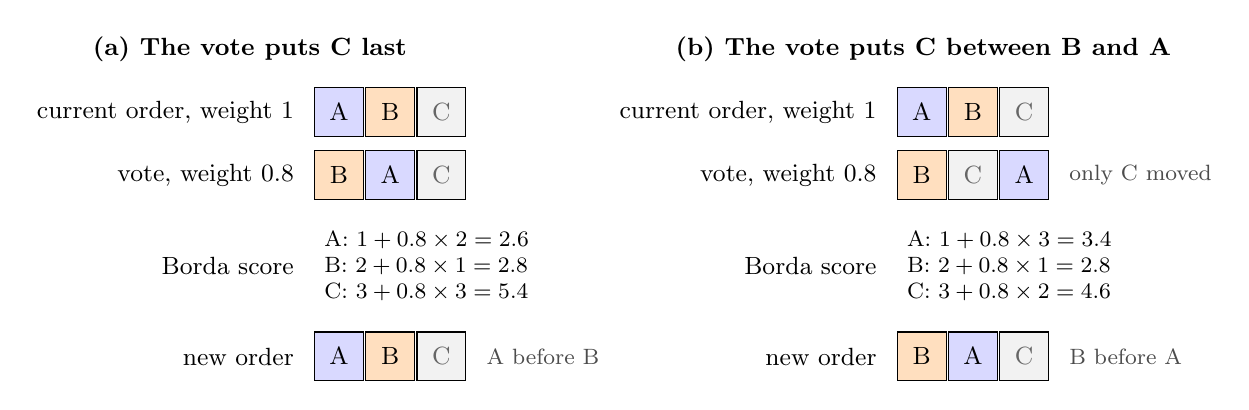
\begin{tikzpicture}[
    >=Stealth,
    lbl/.style={font=\small, anchor=east},
    note/.style={font=\footnotesize, anchor=west, text=black!70},
    cell/.style={draw, minimum width=0.62cm, minimum height=0.62cm, font=\small, inner sep=0pt},
    acell/.style={cell, fill=blue!15},
    bcell/.style={cell, fill=orange!25},
    ccell/.style={cell, fill=black!5, text=black!60},
    score/.style={font=\footnotesize, anchor=west, align=left},
]
% ----- (a) item C last in the vote
\begin{scope}
\node[font=\small\bfseries, anchor=west] at (0.2,0.8) {(a) The vote puts C last};
\node[lbl] at (3.0,0) {current order, weight $1$};
\node[acell] at (3.45,0) {A}; \node[bcell] at (4.1,0) {B}; \node[ccell] at (4.75,0) {C};
\node[lbl] at (3.0,-0.8) {vote, weight $0.8$};
\node[bcell] at (3.45,-0.8) {B}; \node[acell] at (4.1,-0.8) {A}; \node[ccell] at (4.75,-0.8) {C};
\node[lbl] at (3.0,-1.95) {Borda score};
\node[score] at (3.14,-1.95) {A: $1+0.8\times2=2.6$\\B: $2+0.8\times1=2.8$\\C: $3+0.8\times3=5.4$};
\node[lbl] at (3.0,-3.1) {new order};
\node[acell] at (3.45,-3.1) {A}; \node[bcell] at (4.1,-3.1) {B}; \node[ccell] at (4.75,-3.1) {C};
\node[note] at (5.2,-3.1) {A before B};
\end{scope}
% ----- (b) item C between B and A in the vote
\begin{scope}[xshift=7.4cm]
\node[font=\small\bfseries, anchor=west] at (0.2,0.8) {(b) The vote puts C between B and A};
\node[lbl] at (3.0,0) {current order, weight $1$};
\node[acell] at (3.45,0) {A}; \node[bcell] at (4.1,0) {B}; \node[ccell] at (4.75,0) {C};
\node[lbl] at (3.0,-0.8) {vote, weight $0.8$};
\node[bcell] at (3.45,-0.8) {B}; \node[ccell] (cmoved) at (4.1,-0.8) {C}; \node[acell] at (4.75,-0.8) {A};
\node[note] at (5.2,-0.8) {only C moved};
\node[lbl] at (3.0,-1.95) {Borda score};
\node[score] at (3.14,-1.95) {A: $1+0.8\times3=3.4$\\B: $2+0.8\times1=2.8$\\C: $3+0.8\times2=4.6$};
\node[lbl] at (3.0,-3.1) {new order};
\node[bcell] at (3.45,-3.1) {B}; \node[acell] at (4.1,-3.1) {A}; \node[ccell] at (4.75,-3.1) {C};
\node[note] at (5.2,-3.1) {B before A};
\end{scope}
\end{tikzpicture}
\caption{\textbf{A third item changes the order of two.} Two batch updates of one filter over the items A, B and C by the weighted Borda count~\eqref{eq:borda-update}. In each, the filter's current order votes with weight~1 and one vote of weight~0.8 arrives, which meets the weight condition of Proposition~\ref{prop:borda-iia}. A single vote in ArrowFlow weighs less than 0.4 (Section~S1.1), so this vote stands for a few identical votes of one batch. An item's score is its weighted sum of positions, and the new order sorts the scores from lowest to highest. In both updates the current order puts A before B, and the vote puts B before A. The vote differs only in where it places C. Moving C between B and A raises the vote's count of items between them from zero to one. That raises A's score from 2.6 to 3.4 and leaves B's at 2.8, so the new order of A and B reverses. This is one instance of the violation of independence of irrelevant alternatives that Proposition~\ref{prop:borda-iia} guarantees. With the current order held fixed, this update lies in the middle range of Figure~S1, where the violation follows directly.}
\label{fig:iia}
\end{figure}


The proposition fixes the voters and their weights, which in training depend on the predictions. It also treats the prior as a ballot that can change. It concerns every possible profile, and it does not say which profiles arise in training. An actual update holds the current order fixed and maps the votes of a batch to a new filter. In ArrowFlow's layers the votes of one batch weigh less than $V-1$ in total, so this map is not Pareto efficient. Arrow's theorem therefore says nothing about it. The map still violates independence whenever its votes can move the filter. A direct construction shows this (Section~S1.1). So this context dependence lives in the learning rule. The forward pass has none within one layer. Each filter's distance depends only on the input and that filter, so no third filter can reverse the order of two others. A filter's position in the output still depends on all the filters of its layer. And Arrow's theorem predicts nothing about accuracy. The update rule is context dependent whether or not that helps classification.

\paragraph{Three exchangeable stages.}
The voting reading shows three stages where another aggregation rule could be used. They are the filter update, the readout and the vote across views. Arrow's theorem concerns only the first, since the other two output a class.
\begin{enumerate}[leftmargin=2em,topsep=2pt,itemsep=1pt]
  \item The filter update uses the Borda count. One alternative is the footrule median, the permutation with the smallest summed footrule distance to the voters \citep{dwork2001rank}.
  \item The readout takes a plurality vote among the nearest stored training rankings. Its alternatives are the prototype readout and a readout with several prototypes per class, each built by a Borda count.
  \item The $K$ views (Section~\ref{sec:encoding}) are combined by majority vote. With the prototype readout, a Borda count over their class rankings can replace it (Section~\ref{sec:ensemble}).
\end{enumerate}
Sections~\ref{sec:components} and~\ref{sec:controlled} and Section~S4 report these comparisons. The readout with several prototypes per class was compared on inner folds only.

% Supplement subsections typed below as "Section~S<n>.<m>"; build.sh checks each number against the built supplement.
% supplement-ref supp:encoder=S2.3
% supplement-ref supp:learned-method=S6.1
\section{From Real-Valued Data to Permutations: Encoding and Multi-View Ensembles}\label{sec:encoding}

ArrowFlow ranks items, so real-valued features must first become rankings. Sorting a vector keeps only the order of its coordinates and throws away their sizes. For example, $[1.0,2.0,3.0]$ and $[0.01,100,100.01]$ give the same ranking. The encoder therefore first creates more coordinates to compare, by polynomial expansion and projection, and only then sorts. Several differently projected views then vote, and the experiments measure whether all this helps prediction.

\subsection{Encoding}\label{sec:encoder}

An encoder maps $x\in\R^d$ to a score vector $z\in\R^e$ and returns $\pi_x=\argsort(z)$, the ranking of the $e$ coordinate IDs by ascending score. It runs the four steps below, and every statistic they use is fitted on the training rows only.
\begin{enumerate}[leftmargin=2em,topsep=2pt,itemsep=1pt]
\item \emph{Imputation} replaces a missing value by the training mean of its column.
\item \emph{Polynomial expansion} of degree $p$ replaces $x$ by the vector $\phi(x)\in\R^{d'}$ of all monomials of degree at most $p$ in its coordinates, powers included. These monomials let the sorted scores depend on interactions between features, which changes the set of rankings that the encoder can produce from $\R^d$.
\item \emph{Standardization} centers every column and scales each nonconstant column to unit variance, giving $q(x)$.
\item \emph{Projection} multiplies by a matrix $W\in\R^{d'\times e}$, $z=q(x)W$, drawn by one of three strategies. A \emph{random} projection has independent standard normal entries. A \emph{target-aware} projection places coordinates of a linear discriminant analysis (LDA) before random coordinates. LDA is a linear map fitted on the training rows and their labels to separate the classes. A \emph{calibrated} projection is a random projection whose coordinates are standardized before sorting, so that no coordinate dominates through its variance.
\end{enumerate}
Section~S2.3 gives the exact rules of each step. At degree one the encoder also ignores scale. Sliding an example toward the training mean or away from it, along the ray from the mean through the example, leaves all of its rankings unchanged. Only its direction from the mean counts (Section~S2.3).

\subsection{Multi-View Ensemble}\label{sec:ensemble}

Different projection matrices rank the same input differently, and the ensemble uses this diversity (Figure~\ref{fig:pipeline}). A \emph{view} is one encoder together with the network trained on its rankings. ArrowFlow trains $K$ views independently, each from its own seed. View $k$ takes the projection strategy at position $k$ of the repeating cycle target-aware, random, calibrated.

Each view predicts with its nearest-neighbor readout (Section~\ref{sec:prediction}), and a \emph{majority vote} combines the views. The class predicted by the most views wins, even without an absolute majority, and the lowest class ID wins a tie. With the prototype readout, a \emph{Borda count} over the class rankings $\pi^{(L)}$ can replace the vote, as in classifier combination \citep{ho1994decision,vanerp2000variants}.

\subsection{Augmentation}\label{sec:augmentation}

Augmentation adds slightly perturbed copies of the training rankings, the permutation analog of small additive noise. Each copy swaps between $1$ and $s_{\max}$ random pairs of neighboring items, so it lies within footrule distance $2s_{\max}$ of its original. The originals and the validation rankings are kept unchanged. Whether augmentation is switched on is decided from the training rows alone (Section~S2.3).

\subsection{Settings}\label{sec:settings}

The encoded vocabulary size $e$, the degree $p$, the widths, the initial learning rate and the augmentation switch are set from the training rows alone. Some follow a fixed rule, and the others are chosen by an inner cross-validation.

Section~\ref{sec:protocol} describes the selection, and Section~S2 lists every setting with its symbol and value.

\subsection{An Encoder Trained by the Ranking Signal}\label{sec:learned-encoder}

The encoder above is fixed. Nothing in it changes when the network makes a mistake. This subsection replaces it by an \emph{encoder network}, a small neural network whose output scores are sorted exactly as before. It trains that network with motions of the same kind as those that train ArrowFlow's hidden layers. This is an extension of ArrowFlow, and it works in two stages. First, each view's encoder network is trained with its own layer of class filters. Second, the network is fixed and its class filters are set aside. ArrowFlow then trains its ranking layers on the rankings of the trained encoder, as it does with the fixed encoder. The signal that trains the encoder network also has an \emph{away term}, which pushes each coordinate away from the nearest wrong class filter. ArrowFlow's output vote never does that.

The difficulty is the sort. A neural network learns from gradients, but a ranking has no useful gradient. Nudging a score slightly either leaves the ranking unchanged or makes it jump. The motions offer another route (Figure~\ref{fig:target}). They say where each coordinate should sit in the ranking, and a position in the ranking corresponds to a score. So each motion can be translated into a target score, and the network can regress toward it.

The encoder network maps $x$ to scores $h\in\R^e$, and the input ranking is $\pi_x=\orderdesc(h)$, the $e$ coordinates in order of decreasing score. The fixed encoder of Section~\ref{sec:encoder} sorts in increasing order. Here the order is decreasing, so that position 1 holds the largest score. A ranking layer with one filter per class reads $\pi_x$, and its filters keep learning by the output layer's rule of Section~\ref{sec:training}. For an accepted example, the filter $r_y$ of the true class gives each coordinate a motion $m_y=m_{\pi_x\to r_y}$ by~\eqref{eq:motion}. The filter $r_w$ of the nearest wrong class, the other class whose filter lies nearest to $\pi_x$ by the footrule, gives it another motion $m_w=m_{\pi_x\to r_w}$. Coordinate by coordinate, $m_y$ is the motion that the class filter's vote returns (Section~\ref{sec:accumulation}), seen from the input's side and so with the opposite sign. Section~S6.1 gives the exact gating. The \emph{target conversion} turns these motions into numbers in two steps. First, it picks a target position. This is the coordinate's position in the true filter, minus half the displacement that the nearest wrong filter asks of it. Second, it reads the target score off the current scores. The target score is the score that now stands at the resulting position $q_p$,
\begin{equation}\label{eq:target}
\tilde h_{\pi_x[p]} = h_{\pi_x[q_p]},\qquad q_p = p+m_y[p]-\tfrac12\,m_w[p],
\end{equation}
with $q_p$ kept inside $[1,e]$ and the score interpolated between the two nearest positions. In position space, $q_p$ is one gradient step of unit size on a squared loss. It pulls each coordinate toward its position in the true filter and pushes it half as hard away from its position in the nearest wrong filter. Learning vector quantization moves its prototypes by a similar pull and push \citep{kohonen1990self}. The network then takes one step of Adam \citep{kingma2015adam}, a standard method of gradient-based training, on $\tfrac12\lVert h-\tilde h\rVert^2$, averaged over the accepted examples of the batch. The target is held fixed during the step. The sort itself is never differentiated. The discrete motion becomes a target in the network's own units, which is the idea of target propagation \citep{bengio2014auto,lee2015difference}.

% Figure: how the ranking signal trains the encoder network (Section 5.5). Drawn by hand; the scores in panel (b) are an
% illustration of Equation eq:target, not run data: e = 6, the coordinate at p = 5, its position 2 in the true filter
% (m_y = -3) and 6 in the nearest wrong filter (m_w = +1), so q_p = 5 - 3 - 1/2 = 1.5 and the target is (2.1 + 1.4)/2.
\begin{figure}[!htbp]
\centering
\resizebox{\textwidth}{!}{%
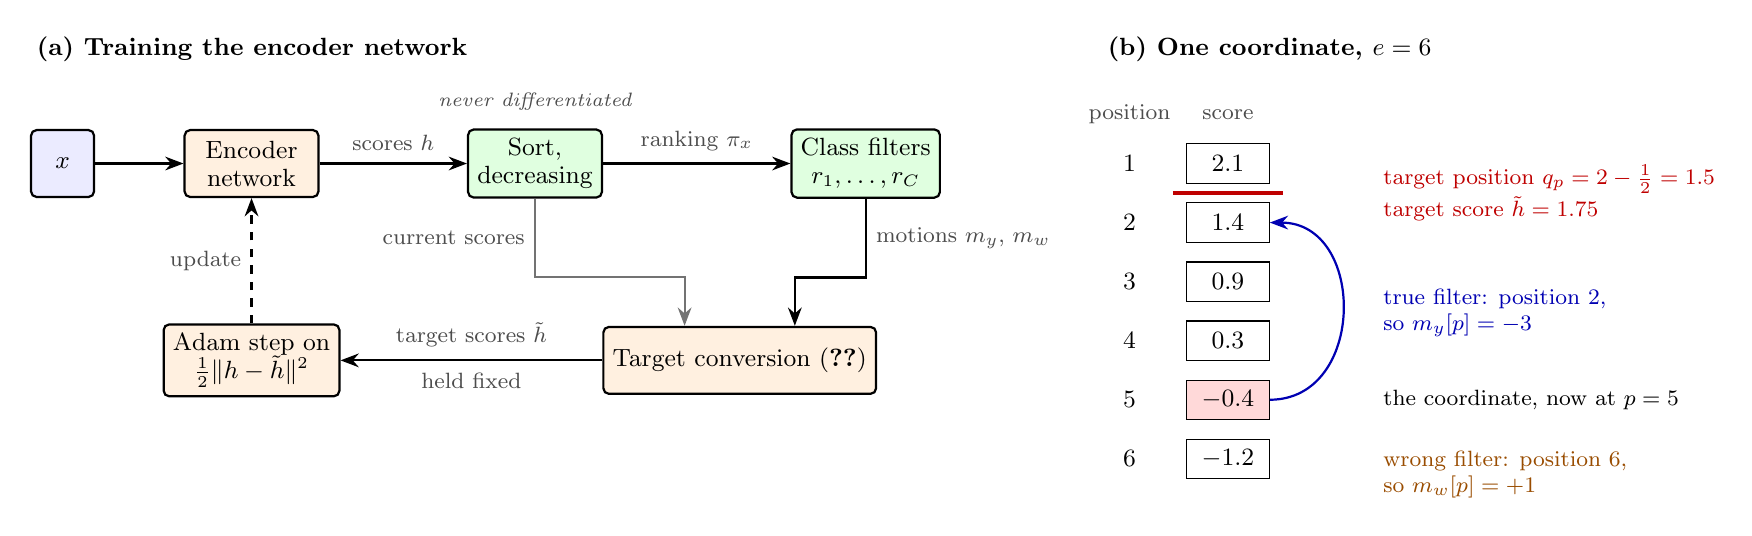
\begin{tikzpicture}[
    >=Stealth,
    box/.style={draw, rounded corners=2pt, minimum height=0.85cm, minimum width=1.7cm,
                font=\small, align=center, thick},
    databox/.style={box, fill=blue!8, minimum width=0.8cm},
    procbox/.style={box, fill=orange!12},
    sortbox/.style={box, fill=green!12},
    arr/.style={->, thick},
    lbl/.style={font=\footnotesize, text=black!70},
    slot/.style={draw, minimum width=1.05cm, minimum height=0.5cm, font=\small, inner sep=0pt},
    note/.style={font=\footnotesize, anchor=west, align=left},
]
% ------------------------------------------------ (a) the training loop
\node[font=\small\bfseries, anchor=west] at (-0.45,1.45) {(a) Training the encoder network};
\node[databox] (x) at (0,0) {$x$};
\node[procbox] (enc) at (2.4,0) {Encoder\\[-1pt]network};
\node[sortbox] (sort) at (6.0,0) {Sort,\\[-1pt]decreasing};
\node[sortbox] (filt) at (10.2,0) {Class filters\\[-1pt]$r_1,\dots,r_C$};
\draw[arr] (x) -- (enc);
\draw[arr] (enc) -- node[lbl, above=1pt] {scores $h$} (sort);
\draw[arr] (sort) -- node[lbl, above=1pt] {ranking $\pi_x$} (filt);
\node[lbl, font=\scriptsize\itshape] at (6.0,0.78) {never differentiated};
\node[procbox] (conv) at (8.6,-2.5) {Target conversion~\eqref{eq:target}};
\node[procbox] (step) at (2.4,-2.5) {Adam step on\\[-1pt]$\tfrac12\lVert h-\tilde h\rVert^2$};
\draw[arr] (filt.south) -- node[lbl, right] {motions $m_y$, $m_w$} ++(0,-1.0) -| ([xshift=7mm]conv.north);
\draw[arr, black!55] (sort.south) -- node[lbl, left] {current scores} ++(0,-1.0) -| ([xshift=-7mm]conv.north);
\draw[arr] (conv) -- node[lbl, above=1pt] {target scores $\tilde h$} node[lbl, below=1pt] {held fixed} (step);
\draw[arr, dashed] (step) -- node[lbl, left] {update} (enc);
% ------------------------------------------------ (b) one coordinate
\begin{scope}[xshift=13.9cm]
\node[font=\small\bfseries, anchor=west] at (-0.75,1.45) {(b) One coordinate, $e=6$};
\node[lbl] at (-0.35,0.62) {position};
\node[lbl] at (0.9,0.62) {score};
\foreach \p/\s in {1/2.1, 2/1.4, 3/0.9, 4/0.3, 5/{-0.4}, 6/{-1.2}} {
  \node[font=\small] at (-0.35,0.75-0.75*\p) {\p};
  \node[slot] (s\p) at (0.9,0.75-0.75*\p) {$\s$};
}
\node[slot, fill=red!15] at (s5) {$-0.4$};
% to the position in the true filter, then half a step away from the wrong filter
\draw[arr, blue!70!black] (s5.east) to[out=0, in=0, looseness=1.4] (s2.east);
\draw[red!75!black, line width=1.6pt] (0.2,-0.375) -- (1.6,-0.375);
\node[note, text=red!75!black] at (2.75,-0.375) {target position $q_p=2-\tfrac12=1.5$\\target score $\tilde h=1.75$};
\node[note, text=blue!70!black] at (2.75,-1.9) {true filter: position 2,\\so $m_y[p]=-3$};
\node[note] at (2.75,-3.0) {the coordinate, now at $p=5$};
\node[note, text=orange!60!black] at (2.75,-3.95) {wrong filter: position 6,\\so $m_w[p]=+1$};
\end{scope}
\end{tikzpicture}%
}
\caption{\textbf{How the ranking signal trains the encoder network.} (a)~The encoder network turns an example $x$ into scores $h$, and a sort in decreasing order gives the input ranking $\pi_x$. A ranking layer with one filter per class reads $\pi_x$ and keeps learning by its own vote. For an accepted example, the filter of the true class and the filter of the wrong class nearest to $\pi_x$ give the motions $m_y$ and $m_w$. The target conversion~\eqref{eq:target} turns them into target scores $\tilde h$. With $\tilde h$ held fixed, an Adam step on $\tfrac12\lVert h-\tilde h\rVert^2$ updates the network (dashed arrow). No gradient passes through the sort. After training, each view's encoder network is fixed and replaces that view's fixed encoder. (b)~The conversion for one coordinate, with $e=6$ scores listed from the largest down. The coordinate sits at position $p=5$ with score $-0.4$. The true filter puts it at position 2, so $m_y[p]=-3$ (blue arrow), and the nearest wrong filter puts it at position 6, so $m_w[p]=+1$. Its target position is $q_p=5-3-\tfrac12=1.5$ (red line). Its target score, $1.75$, lies halfway between the scores at positions 1 and 2, and the loss pulls its score toward that value. The scores are made up for the example.}
\label{fig:target}
\end{figure}


The encoder network has three fully connected layers of width $e$, and the first two start with weights drawn uniformly from 0 to 1. It trains for 60 passes over the training rows, with no validation checkpoint. Section~\ref{sec:learned} evaluates the extension, and Section~S6.1 gives every setting.

% Supplement subsections typed below as "Section~S<n>.<m>"; build.sh checks each number against the built supplement.
% supplement-ref supp:gaussian=S1.3
% supplement-ref supp:alphabet=S1.5
% supplement-ref supp:angle=S1.6
% supplement-ref supp:margin=S1.7
% supplement-ref supp:borda=S1.8
% supplement-ref supp:persistent=S1.9
\section{Theoretical Analysis}\label{sec:theory}

What do the fixed parts of ArrowFlow guarantee? This section answers four questions.
\begin{enumerate}[leftmargin=2em,topsep=2pt,itemsep=1pt]
\item When does the encoded ranking stay the same?
\item Which rankings can the encoder produce?
\item How far can an input move before a fixed layer changes its output?
\item What does one batch update compute?
\end{enumerate}
Each statement concerns a fixed encoder, layer or batch. None of them is a convergence or generalization theorem for the trained network. Section~S1 states and proves every result that we summarize here in words.

\subsection{Stability of the Ordinal Encoding}\label{sec:theory-stability}

The encoded ranking $\pi_x=\argsort(z)$ changes only when two coordinates of the score vector $z\in\R^e$ (Section~\ref{sec:encoding}) cross. So the smallest gap between two scores, $\delta_{\min}(z)=\min_{i<j}|z_i-z_j|$, controls how stable the ranking is.

\begin{proposition}[Score-gap stability]\label{prop:score-stability}
Let $z\in\R^e$, $e\ge2$, have distinct coordinates, and let $\varepsilon\in\R^e$ satisfy $\|\varepsilon\|_\infty<\delta_{\min}(z)/2$. Then $\argsort(z+\varepsilon)=\argsort(z)$.
\end{proposition}

In words, if every score moves by less than half the smallest gap, the ranking stays the same. The condition is sufficient but not necessary. Its bound cannot be raised, because the two closest scores cross when each moves toward the other by more than half their gap (Figure~\ref{fig:cones}b). Nor does it give a noise threshold, because Gaussian noise exceeds any bound with positive probability. For Gaussian input noise and an encoder of degree one, Section~S1.3 bounds the probability that the ranking changes.

\subsection{The Ordinal Alphabet}\label{sec:theory-alphabet}

Ranking keeps order and discards magnitude, so the encoder can output at most $e!$ rankings. All score vectors without ties that share one ranking $\pi$ form an open convex cone, $\{z: z_{\pi[1]}<z_{\pi[2]}<\dots<z_{\pi[e]}\}$, cut out by the hyperplanes $z_i=z_j$ (Figure~\ref{fig:cones}). A vector with tied scores lies on a wall of a cone and gets the ranking that the ID rule assigns. The encoding is constant inside a cone and jumps at its walls. A fixed projection may land in only some of these cones. So $e!$ bounds the alphabet of rankings that the encoder can emit, but it does not measure the information the data carry (Section~S1.5).

At degree one the alphabet can be counted. Every score is then the dot product of the $d$ standardized features with a fixed vector of the view, a column of $W$ for a random view. So the ranking orders $e$ fixed points in $d$ dimensions by their projection onto one direction. \citet{cover1967orderings} counted how many orderings such projections can produce. A view of degree one reaches at most that many rankings, and a random view can reach all of them. For $e=16$ and $d=4$ there are 437,040, against $16!\approx2.1\times10^{13}$ (Section~S1.5). Polynomial expansion makes the scores linear in more coordinates, so it can enlarge this set.

For the random projection, inputs that point in similar directions get similar rankings. Suppose that the expanded, standardized features of two fixed inputs form the angle $\theta$. Then, in expectation over the random projection matrix, their rankings disagree on $\binom{e}{2}\theta/\pi$ coordinate pairs (Section~S1.6).

\begin{figure}[!htbp]
\centering
\resizebox{0.55\textwidth}{!}{%
\begin{tikzpicture}[scale=1.0]
\node[font=\small, anchor=west] at (-4.6, 3.9) {(a)};
\node[font=\scriptsize, anchor=west] at (-3.9, 3.9) {section $z_1{+}z_2{+}z_3=0$};
% The three walls {z_i = z_j} all contain the diagonal z_1=z_2=z_3, so in a transverse
% section they are three concurrent lines through the origin, 60 degrees apart, and they
% cut the section into exactly six sectors, one per ordering of three coordinates.
% one dash style per wall, so that the walls differ by more than color
\draw[dashed, thick, blue!70] (0, -4.2) -- (0, 4.2) node[above, font=\scriptsize, blue!80!black] {$z_1{=}z_2$};
\draw[dash dot, thick, green!50!black] (-3.637, -2.1) -- (3.637, 2.1) node[right, font=\scriptsize, green!50!black] {$z_2{=}z_3$};
\draw[dash dot dot, thick, red!70] (3.637, -2.1) -- (-3.637, 2.1) node[left, font=\scriptsize, red!80!black] {$z_1{=}z_3$};
\fill[black!45] (0,0) circle (1.6pt);
% Sector labels, counter-clockwise from the 0 degree direction
\node[font=\scriptsize, fill=white, inner sep=2pt, rounded corners=2pt] at (4.5, -0.55) {$z_1{>}z_3{>}z_2$};
\node[font=\scriptsize, fill=white, inner sep=2pt, rounded corners=2pt] at (1.45, 2.512) {$z_1{>}z_2{>}z_3$};
\node[font=\scriptsize, fill=white, inner sep=2pt, rounded corners=2pt] at (-1.45, 2.512) {$z_2{>}z_1{>}z_3$};
\node[font=\scriptsize, fill=white, inner sep=2pt, rounded corners=2pt] at (-2.9, 0) {$z_2{>}z_3{>}z_1$};
\node[font=\scriptsize, fill=white, inner sep=2pt, rounded corners=2pt] at (-1.45, -2.512) {$z_3{>}z_2{>}z_1$};
\node[font=\scriptsize, fill=white, inner sep=2pt, rounded corners=2pt] at (1.45, -2.512) {$z_3{>}z_1{>}z_2$};
% Data point and stability circle, drawn to scale. The centered point (1,-1,0) sits on the
% 0 degree ray at distance sqrt(2) from the origin; its nearest wall is at 1/sqrt(2), so with
% delta_min(z) = 1 the certified radius 1/2 is 0.707 of that distance.
\fill[black] (2.6, 0) circle (2pt);
\draw[thick, dotted, black!40] (2.6, 0) circle (0.919);
\draw[black!50] (2.6, 0) -- (1.681, 0);
\node[font=\scriptsize, black!75, anchor=north] at (2.14, -0.07) {$\delta_{\min}(z)/2$};
\node[font=\scriptsize, anchor=west] at (3.6, 1.1) {$z = (3, 1, 2)$};
\node[font=\scriptsize, anchor=west, black!75] at (3.6, 0.7) {$\argsort(z) = [2,3,1]$};
\end{tikzpicture}%
}\\[8pt]
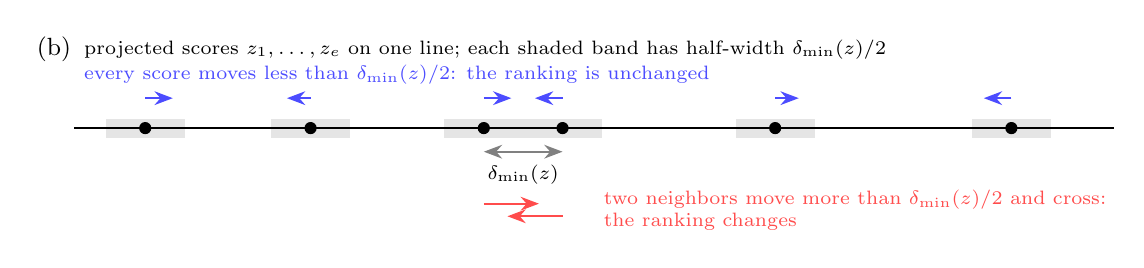
\begin{tikzpicture}[>=Stealth, lbl/.style={font=\scriptsize}]
\node[font=\small, anchor=west] at (-0.6, 1.6) {(b)};
% one number line of e projected scores; shaded: the certified radius delta_min/2 around each score
\node[lbl, anchor=west] at (0.0, 1.6) {projected scores $z_1, \dots, z_e$ on one line; each shaded band has half-width $\delta_{\min}(z)/2$};
\foreach \x in {0.9, 3.0, 5.2, 6.2, 8.9, 11.9} {
    \fill[black!10] (\x-0.5, 0.48) rectangle (\x+0.5, 0.72);
}
\draw[thick] (0.0, 0.6) -- (13.2, 0.6);
\foreach \x in {0.9, 3.0, 5.2, 6.2, 8.9, 11.9} {
    \fill (\x, 0.6) circle (2.2pt);
}
% a perturbation inside the radius: every score stays in its band, the ranking is unchanged
\node[lbl, blue!70, anchor=west] at (0.0, 1.28) {every score moves less than $\delta_{\min}(z)/2$: the ranking is unchanged};
\foreach \x/\d in {0.9/0.35, 3.0/-0.3, 5.2/0.35, 6.2/-0.35, 8.9/0.3, 11.9/-0.35} {
    \draw[->, thick, blue!70] (\x, 0.98) -- (\x+\d, 0.98);
}
% the smallest gap
\draw[<->, thick, black!50] (5.2, 0.3) -- (6.2, 0.3);
\node[lbl, anchor=north] at (5.7, 0.26) {$\delta_{\min}(z)$};
% a perturbation beyond the radius: two neighbors cross, the ranking changes
\draw[->, thick, red!70] (5.2, -0.36) -- (5.9, -0.36);
\draw[->, thick, red!70] (6.2, -0.52) -- (5.5, -0.52);
\node[lbl, red!70, anchor=west, align=left] at (6.6, -0.44) {two neighbors move more than $\delta_{\min}(z)/2$ and cross:\\ the ranking changes};
\end{tikzpicture}
\caption{\textbf{Permutation cones and the stability radius.} (a)~Up to the hyperplanes $\{z_i=z_j\}$, whose points the tie rule assigns, the argsort encoding partitions the projected space $\R^e$ into $e!$ open convex cones (Weyl chambers). They are drawn here for $e=3$ in the plane $z_1+z_2+z_3=0$, which every cone meets and which the three hyperplanes cut into six sectors. All points in a cone map to the same permutation. The point $z=(3,1,2)$ is drawn at its position in the plane, which differs from $z$ by a multiple of the all-ones vector and has the same ranking and the same coordinate gaps. The dotted circle has radius $\delta_{\min}(z)/2$, half the smallest coordinate gap of Proposition~\ref{prop:score-stability}. It lies inside the region $\|\varepsilon\|_\infty<\delta_{\min}(z)/2$, so a perturbation inside it cannot cross a boundary. The nearest wall is farther away, at distance $\delta_{\min}(z)/\sqrt2$. (b)~The same condition on one line of projected scores. Scores that each move by less than $\delta_{\min}(z)/2$ keep their ranking, and two neighbors that move further can cross.}
\label{fig:cones}
\end{figure}


\subsection{Margins and Ties of a Fixed Ranking Layer}\label{sec:theory-margin}

A fixed layer is stable in the same way. The footrule is a metric, so no filter's distance changes by more than the input moves. When all distances differ, the smallest gap between consecutive distances therefore guarantees the same output for every input within half that gap (Section~S1.7). The guarantee fails where distances tie. Footrule distances are even integers up to $\lfloor V^2/2\rfloor$ \citep{diaconis1977footrule}, so at most $\lfloor V^2/4\rfloor+1$ values occur. A layer with more filters than that has tied distances at every input. For example, a layer of $128$ filters over $V=16$ items can see at most $65$ distinct distances. Ties are common well before that bound. The distances from an input to random filters crowd around their mean $(V^2-1)/3$ with a standard deviation near $0.21\,V^{3/2}$. At the hidden-layer sizes used here, random filters therefore leave almost no input with all distances distinct, and the guarantee then covers at most the nearest filter (Section~S1.7). Where distances tie, the tie rule of Section~\ref{sec:forward} decides the output order.

\subsection{What One Batch Update Computes}\label{sec:theory-aggregation}

One batch update is a weighted Borda count of the accepted votes and the prior. In general it is not the footrule median. Because the accumulator is reset after every batch, it keeps no running estimate of where each item belongs on average. Each update depends only on the filter's current order and the current batch. With little vote weight, the current order can even hold against the average vote (Section~S1.9).

\begin{proposition}[One batch update is a weighted Borda count]\label{prop:batch-borda}
Fix a filter $r_j$ and the targets $\tilde\tau_1,\dots,\tilde\tau_n$ of one batch with vote weights $|a_1|,\dots,|a_n|>0$. After accumulation, the mean voted position $s_p$ of~\eqref{eq:rowmean} for the row $p=\operatorname{pos}_{r_j}(v)$ of item $v$ equals
\begin{equation}\label{eq:rowmean-borda}
s_p=\frac{\operatorname{pos}_{r_j}(v)+\sum_{t=1}^{n}|a_t|\operatorname{pos}_{\tilde\tau_t}(v)}{1+\sum_{t=1}^{n}|a_t|}=\frac{P_j(v)}{1+\sum_{t=1}^{n}|a_t|},
\end{equation}
so in exact arithmetic the reordered filter is the ranking by $P_j$ of~\eqref{eq:borda-update} with the fixed tie rule. It differs in general from the footrule median of the same profile, even when the mean positions are distinct.
\end{proposition}

The weighted footrule median minimizes the summed absolute position differences to the voters, and minimum-cost matching computes it exactly \citep{dwork2001rank}. The Borda ranking instead minimizes the summed squared differences. The profiles of Section~S1.8 show that the two rules do disagree, on a finite profile and in the limit. Picture an idealized estimator that kept every vote drawn from one fixed distribution. It would converge to the ranking by expected position when the expected positions differ. The reset update need not converge to it, and in the network the votes also change with the current predictions (Section~S1.9).

% Supplement subsections and tables typed below as "Section~S<n>.<m>" and "Table~S<n>"; build.sh checks each number
% against the built supplement.
% supplement-ref supp:angle=S1.6
% supplement-ref supp:settings=S2.4
% supplement-ref supp:statistics=S2.5
% supplement-ref supp:selection=S3.1
% supplement-ref supp:benchmark=S3.2
% supplement-ref supp:training=S3.3
% supplement-ref supp:sorting=S3.4
% supplement-ref supp:motion=S3.6
% supplement-ref supp:controlled=S3.7
% supplement-ref supp:ablation-arrowflow=S4.1
% supplement-ref supp:datasets=S5.2
% supplement-ref supp:learned-development=S6.2
% supplement-ref supp:learned-nested=S6.3
% supplement-ref supp:learned-swap=S6.4
% supplement-ref tab:s-motion-scramble=S28
% supplement-ref tab:s-motion-purity=S29
\section{Experiments}\label{sec:experiments}

The experiments ask six questions.
\begin{enumerate}[leftmargin=2em,topsep=2pt,itemsep=1pt]
\item How accurate is ArrowFlow next to standard classifiers tuned in the same way?
\item Does training the ranking filters help, compared with leaving them in their random starting orders?
\item What does each part of the method contribute?
\item Is it the particular signal sent down from the output layer that helps, or would any movement of the filters do?
\item What does training change inside the network, and where does its benefit stop?
\item Can motions of the same kind train a real-valued encoder network, and does ArrowFlow gain from it?
\end{enumerate}

In brief, ArrowFlow trails the best tuned classical model on all seventeen datasets, and training adds only a modest gain. The signal that training sends down does carry information. Yet a fixed kernel on rankings from the same encoder family is more accurate on most datasets. So the paper's contribution is the learning rule itself. Motions of the same kind also train a real-valued encoder network. With the trained encoder, ArrowFlow has the higher mean accuracy on 11 of the 17 datasets, significantly on one.

\subsection{How We Tested}\label{sec:protocol}

A fair test needs two things. It needs datasets that did not shape the method, and it needs a way of choosing settings that never looks at the test data. Section~S2.5 gives the complete protocol. The author used generative artificial intelligence tools for software development, running and analyzing the experiments, and editing the manuscript, and reviewed all of their output. The tools were Claude Opus 5, Claude Opus 5.5, Claude Fable 5 and Claude Fable 5.1 (Anthropic), and GPT 5.6 Sol and GPT 6 Astra (OpenAI).

\paragraph{Datasets.} We use seventeen classification datasets. Seven are standard benchmarks from the University of California, Irvine (UCI) Machine Learning Repository \citep{dua2019uci}, and they served during the method's development. They are Iris \citep{uci_iris}, Wine \citep{uci_wine}, Breast cancer \citep{uci_wdbc}, Wine quality (red wines, three quality classes) \citep{uci_winequality}, Vehicle \citep{uci_vehicle}, Segment \citep{uci_segment} and Digits \citep{uci_digits}. Wine quality's three classes are the quality scores 5 or less, 6, and 7 or more. The other ten, the further datasets, were fixed in advance as every dataset of a predefined pool of OpenML datasets \citep{vanschoren2014openml} that met prespecified eligibility rules, as interpreted during selection and before any model was fitted (Section~S3.1). They are balance-scale \citep{uci_balance}, mfeat-zernike \citep{uci_mfeat}, ionosphere \citep{uci_ionosphere}, vertebra-column \citep{uci_vertebral}, diabetes \citep{smith1988diabetes}, banknote-authentication \citep{uci_banknote}, qsar-biodeg \citep{uci_qsar}, steel-plates-fault \citep{uci_steel}, climate-model-simulation-crashes \citep{uci_climate} and the hepatitis C virus (HCV) data \citep{uci_hcv}. The method, its candidate settings and the comparison models were fixed before these ten were selected, and none of the ten had been used in the method's earlier development (Section~S5). The encoder network of Section~\ref{sec:learned-encoder} is an exception. Its target conversion and settings were developed on single splits of twelve of the seventeen datasets, six of them further datasets (Section~S6.2). All seventeen are small: 150 to 2,310 rows, 4 to 64 features and 2 to 10 classes (Section~S5.2).

\paragraph{How settings are chosen.} Every tuned setting is chosen by nested cross-validation, so within a run the test data never influence a choice. Each dataset is split into five parts that keep its class proportions. Each part serves once as the test set, and the split is repeated three times with different shuffles. So every model is tested on the same 15 test sets, called outer folds. All tuning happens inside the other four parts of each split, its training partition \citep{cawley2010selection}. These are split again into three inner folds, and each model picks its configuration there from at most 24 candidates. A stochastic model, one whose fit depends on a random seed, has its three best candidates rescored with all three fitting seeds. The chosen configuration is refitted on the whole training partition and scored once on the test set.

\paragraph{Models.} ArrowFlow always uses $K=7$ views, the nearest-neighbor readout and the validation checkpoint. Its 16 candidates vary the hidden-layer widths, the learning rate and two encoder settings (Section~S2.4). The comparison models are five scikit-learn classifiers \citep{pedregosa2011sklearn}, each tuned in the same way. They are a support vector classifier (SVC) with a radial basis function kernel, a random forest, a multilayer perceptron (MLP), numeric kNN on the standardized raw features and gradient boosting. The majority class gives a baseline. ArrowFlow also chooses its readout's neighbor count and weighting inside every fit, outside the candidate budget.

\paragraph{How differences are judged.} Errors are in percent and differences in percentage points (pp). Tables give each model's mean error over the 15 test sets, with its standard deviation (SD) across them. To compare two models, we take their accuracy difference on each test set and report the mean with a 95\% interval. The 15 splits share training data, so their differences are correlated. We use the corrected resampled $t$ interval, which is wider to allow for that \citep{nadeau2003inference,bouckaert2004evaluating}. Over many datasets some differences look large by chance alone. We therefore correct the $p$ values for the number of comparisons with the Holm method \citep{holm1979simple}, and a difference is significant when its corrected $p$ value is below $0.05$. Each correction covers a group of comparisons that a run protocol fixed before they were scored. Each such protocol was frozen before its run, with its hash and time recorded, but none was deposited with an external registry. Analyses defined afterwards are exceptions, and we call them post hoc. On the seven benchmark datasets, the training comparisons were fixed after ArrowFlow's own results there were known (Section~S2.5).

\subsection{How Accurate Is ArrowFlow?}\label{sec:main-benchmark}

How does ArrowFlow compare with standard classifiers that get the same data, the same folds and the same cap on candidates? Table~\ref{tab:main} gives the test error of every model on every dataset.

ArrowFlow is never the most accurate model. On every one of the seventeen datasets the best tuned classical model has lower error, by $0.19$ (banknote-authentication) to $5.32$ percentage points (ionosphere). Ranked within each dataset and averaged, ArrowFlow comes fourth of the six tuned models, between random forest and gradient boosting. On the ten further datasets alone it comes fifth, ahead of numeric kNN only (Section~S3.2). Accuracy can hide a weakness on a rare class. Balanced accuracy averages, over the classes, the share of each class's rows that a model gets right. On climate-model-simulation-crashes, ArrowFlow's balanced accuracy is 51.2 percent, barely above the 50 percent of the majority class. The support vector classifier reaches 76.1 percent (Section~S3.2).

% Rendered by render_tables.py from run files; do not edit by hand.
\begin{table}[!htbp]
\caption{\textbf{ArrowFlow against five tuned classical models and the majority class on the seventeen datasets.} Mean test error in percent over the 15 outer folds (5 folds $\times$ 3 repeats), with the standard deviation (SD) across folds in parentheses; the SD describes spread, not a confidence interval. Every model chose its configuration on inner folds only (Section~\ref{sec:protocol}). Bold marks the lowest unrounded error among ArrowFlow and the five classical models. The last column gives ArrowFlow's error minus that of the best tuned classical model, the majority class excluded, in percentage points, positive when ArrowFlow trails; it is positive on all seventeen datasets. It is computed from unrounded errors, so it can differ in the last digit from the printed errors; Section~S3.2 lists the errors of the tuned models to two decimals. The marks are post hoc flags. c: the best tuned classical model has less than 1\% error. m: ArrowFlow is within 0.5 points of the majority class, and the best tuned model is at least 2 points better. n: no model has lower error than the majority class. SVC: support vector classifier with a radial basis function (RBF) kernel; MLP: multilayer perceptron; kNN: nearest-neighbor classifier; HCV: hepatitis C virus.}
\label{tab:main}
\centering
\scriptsize
\setlength{\tabcolsep}{3pt}
\resizebox{\ifdim\width>\linewidth\linewidth\else\width\fi}{!}{%
\begin{tabular}{lrrrrrrrr}
\toprule
Dataset & ArrowFlow & SVC (RBF) & Random forest & MLP & Numeric kNN & \begin{tabular}[b]{@{}r@{}}Gradient\\boosting\end{tabular} & \begin{tabular}[b]{@{}r@{}}Majority\\class\end{tabular} & \begin{tabular}[b]{@{}r@{}}Gap to best\\tuned (pp)\end{tabular} \\
\midrule
\multicolumn{9}{l}{\emph{Benchmark datasets}} \\
Iris & 5.0 (3.5) & \textbf{4.0 (3.4)} & 5.3 (4.3) & 4.1 (3.7) & 4.7 (3.3) & 5.6 (3.5) & 66.7 (0.0) & +1.04 \\
Wine & 3.2 (2.9) & \textbf{1.5 (2.3)} & 1.8 (1.6) & 1.9 (2.2) & 3.4 (3.4) & 2.6 (2.5) & 60.1 (1.6) & +1.69 \\
Breast cancer & 2.7 (1.1) & \textbf{2.3 (1.5)} & 4.3 (1.5) & 2.9 (1.5) & 3.5 (1.5) & 3.9 (1.6) & 37.3 (0.4) & +0.33 \\
Wine quality & 27.7 (2.1) & 33.1 (3.4) & \textbf{27.2 (2.3)} & 32.3 (2.6) & 28.8 (2.2) & 30.7 (2.1) & 53.5 (0.1) & +0.47 \\
Vehicle & 19.9 (1.5) & \textbf{16.5 (2.0)} & 25.7 (2.3) & 17.2 (2.0) & 29.3 (2.6) & 24.3 (2.2) & 74.2 (0.3) & +3.40 \\
Segment & 2.6 (0.7) & 3.3 (0.9) & \textbf{1.9 (0.7)} & 2.8 (0.9) & 3.4 (1.1) & 2.1 (0.6) & 85.7 (0.0) & +0.66 \\
Digits & 2.8 (0.9) & \textbf{1.8 (0.6)} & 2.4 (0.7) & 2.3 (0.8) & 2.1 (0.7) & 3.3 (0.9) & 89.9 (0.2) & +0.97 \\
\midrule
\multicolumn{9}{l}{\emph{Further datasets}} \\
balance-scale & 6.0 (1.3) & \textbf{2.1 (1.8)} & 13.8 (2.1) & 2.2 (1.1) & 10.2 (1.5) & 8.4 (0.8) & 54.2 (0.3) & +3.95 \\
mfeat-zernike & 19.3 (1.0) & \textbf{17.1 (1.6)} & 22.3 (2.0) & 18.9 (1.2) & 19.6 (1.7) & 22.4 (1.8) & 90.0 (0.0) & +2.18 \\
ionosphere & 11.2 (3.4) & \textbf{5.9 (2.7)} & 7.0 (2.5) & 8.0 (2.6) & 10.2 (3.5) & 6.6 (2.1) & 35.9 (0.4) & +5.32 \\
vertebra-column & 16.9 (3.6) & \textbf{14.0 (5.2)} & 15.8 (3.2) & 15.4 (4.4) & 19.8 (4.0) & 17.8 (4.3) & 51.6 (0.0) & +2.90 \\
diabetes & 24.0 (2.5) & \textbf{22.7 (2.9)} & 23.9 (2.6) & 23.5 (1.5) & 24.5 (2.7) & 24.0 (3.2) & 34.9 (0.2) & +1.34 \\
banknote-authentication$^{\mathrm{c}}$ & 0.2 (0.5) & 0.0 (0.1) & 0.9 (0.7) & \textbf{0.0 (0.0)} & 0.3 (0.5) & 0.3 (0.3) & 44.5 (0.1) & +0.19 \\
qsar-biodeg & 12.6 (1.8) & 12.2 (3.1) & 13.0 (2.1) & \textbf{12.0 (2.9)} & 13.7 (2.7) & 13.2 (2.5) & 33.7 (0.2) & +0.52 \\
steel-plates-fault & 24.8 (1.5) & 23.9 (2.1) & 21.2 (1.6) & 24.2 (1.7) & 25.5 (1.4) & \textbf{21.0 (1.8)} & 65.3 (0.1) & +3.82 \\
climate-model-simulation-crashes$^{\mathrm{m}}$ & 8.3 (0.6) & \textbf{5.4 (2.2)} & 6.4 (1.1) & 5.6 (1.7) & 6.8 (1.1) & 5.9 (1.4) & 8.5 (0.4) & +2.96 \\
HCV$^{\mathrm{n}}$ & 75.6 (1.7) & 75.5 (2.0) & 75.9 (1.6) & 75.0 (1.8) & \textbf{74.1 (2.6)} & 76.9 (2.4) & 73.9 (0.2) & +1.50 \\
\bottomrule
\end{tabular}
}
\end{table}


\subsection{Does Training Help?}\label{sec:training-controls}

Random ranking filters already turn an input into a new ranking, and the nearest-neighbor readout may work well on it without any training. To see what the learning rule adds, we compare ArrowFlow with two controls that train no filters but are otherwise tuned exactly like it (Table~\ref{tab:training}). The untrained ArrowFlow keeps its random initial filters. Tuned input footrule kNN skips the ranking layers and applies the nearest-neighbor readout directly to the encoded input rankings.

% Rendered by render_tables.py from run files; do not edit by hand.
\begin{table}[!htbp]
\caption{\textbf{What training adds, on the seventeen datasets.} Upper part: mean test error in percent, lower is better, of five classifiers that all predict from nearest neighbors. From left to right they are numeric kNN on the standardized raw features, numeric kNN on the projected scores before sorting, tuned input footrule kNN on the encoded input rankings, the untrained ArrowFlow and ArrowFlow. Neighboring columns differ in more than one component, so this ladder describes and does not decompose. Lower part: ArrowFlow's accuracy minus that of each control in percentage points, positive when ArrowFlow is more accurate, with its 95\% interval, which is not corrected for multiple comparisons. Holm $p$ is corrected over the comparisons named in the block header, which the run protocols fixed before the controls were scored; the benchmark family was fixed after ArrowFlow's own benchmark results were known. $^\ddagger$: still below 0.05 after one post hoc correction over all 34 comparisons. Both controls share ArrowFlow's encoder family but choose their own settings on inner folds. kNN: nearest-neighbor classifier; HCV: hepatitis C virus.}
\label{tab:training}
\centering
\scriptsize
\setlength{\tabcolsep}{3pt}
\begin{tabular}{lrrrrr}
\toprule
Dataset & \begin{tabular}[b]{@{}r@{}}Numeric kNN,\\raw features\end{tabular} & \begin{tabular}[b]{@{}r@{}}Numeric kNN,\\projected scores\end{tabular} & \begin{tabular}[b]{@{}r@{}}Tuned input\\footrule kNN\end{tabular} & \begin{tabular}[b]{@{}r@{}}Untrained\\ArrowFlow\end{tabular} & ArrowFlow \\
\midrule
\multicolumn{6}{l}{\emph{Benchmark datasets}} \\
Iris & 4.7 & 4.0 & 5.6 & 6.0 & 5.0 \\
Wine & 3.4 & 3.9 & 4.9 & 3.9 & 3.2 \\
Breast cancer & 3.5 & 3.3 & 3.6 & 3.2 & 2.7 \\
Wine quality & 28.8 & 28.2 & 28.1 & 27.8 & 27.7 \\
Vehicle & 29.3 & 25.1 & 24.7 & 23.4 & 19.9 \\
Segment & 3.4 & 3.6 & 3.8 & 3.6 & 2.6 \\
Digits & 2.1 & 2.4 & 2.8 & 3.0 & 2.8 \\
\midrule
\multicolumn{6}{l}{\emph{Further datasets}} \\
balance-scale & 10.2 & 10.3 & 10.9 & 11.0 & 6.0 \\
mfeat-zernike & 19.6 & 19.0 & 21.5 & 21.6 & 19.3 \\
ionosphere & 10.2 & 12.3 & 11.2 & 11.4 & 11.2 \\
vertebra-column & 19.8 & 16.7 & 17.8 & 18.0 & 16.9 \\
diabetes & 24.5 & 24.3 & 24.0 & 24.8 & 24.0 \\
banknote-authentication & 0.3 & 0.2 & 0.1 & 0.2 & 0.2 \\
qsar-biodeg & 13.7 & 13.8 & 14.0 & 13.5 & 12.6 \\
steel-plates-fault & 25.5 & 25.4 & 25.2 & 25.6 & 24.8 \\
climate-model-simulation-crashes & 6.8 & 7.6 & 8.3 & 8.4 & 8.3 \\
HCV & 74.1 & 75.6 & 75.7 & 75.2 & 75.6 \\
\bottomrule
\end{tabular}
\par\medskip
\begin{tabular}{lrrrr}
\toprule
Dataset & \begin{tabular}[b]{@{}r@{}}ArrowFlow $-$\\untrained (pp)\end{tabular} & \begin{tabular}[b]{@{}r@{}}Holm\\$p$\end{tabular} & \begin{tabular}[b]{@{}r@{}}ArrowFlow $-$ tuned\\input footrule kNN (pp)\end{tabular} & \begin{tabular}[b]{@{}r@{}}Holm\\$p$\end{tabular} \\
\midrule
\multicolumn{5}{l}{\emph{Benchmark datasets: Holm correction over fourteen comparisons}} \\
Iris & +0.96 [$-$1.35, +3.28] & 1.000 & +0.52 [$-$2.25, +3.29] & 1.000 \\
Wine & +0.74 [$-$1.13, +2.61] & 1.000 & +1.68 [$-$1.04, +4.40] & 1.000 \\
Breast cancer & +0.55 [$-$0.44, +1.53] & 1.000 & +0.88 [$-$0.10, +1.86] & 0.751 \\
Wine quality & +0.11 [$-$1.44, +1.66] & 1.000 & +0.44 [$-$1.23, +2.10] & 1.000 \\
Vehicle & +3.51 [+1.27, +5.74] & 0.060 & +4.81 [+1.86, +7.75] & 0.049 \\
Segment & +1.06 [+0.24, +1.88] & 0.161 & +1.18 [+0.39, +1.97] & 0.075 \\
Digits & +0.22 [$-$0.70, +1.13] & 1.000 & $-$0.03 [$-$1.01, +0.96] & 1.000 \\
\midrule
\multicolumn{5}{l}{\emph{Further datasets: Holm correction over ten comparisons per control}} \\
balance-scale & +4.98 [+3.38, +6.57] & $<$0.001$^\ddagger$ & +4.91 [+2.98, +6.83] & $<$0.001$^\ddagger$ \\
mfeat-zernike & +2.34 [+1.28, +3.40] & 0.003$^\ddagger$ & +2.18 [+1.09, +3.28] & 0.007$^\ddagger$ \\
ionosphere & +0.16 [$-$3.60, +3.92] & 1.000 & $-$0.00 [$-$2.97, +2.97] & 1.000 \\
vertebra-column & +1.08 [$-$2.43, +4.58] & 1.000 & +0.97 [$-$1.52, +3.46] & 1.000 \\
diabetes & +0.71 [$-$1.59, +3.01] & 1.000 & $-$0.03 [$-$1.52, +1.47] & 1.000 \\
banknote-authentication & +0.03 [$-$0.25, +0.31] & 1.000 & $-$0.09 [$-$0.68, +0.50] & 1.000 \\
qsar-biodeg & +0.92 [$-$0.14, +1.97] & 0.663 & +1.42 [+0.45, +2.39] & 0.056 \\
steel-plates-fault & +0.72 [$-$1.23, +2.67] & 1.000 & +0.39 [$-$1.31, +2.08] & 1.000 \\
climate-model-simulation-crashes & +0.02 [$-$0.43, +0.48] & 1.000 & $-$0.04 [$-$0.65, +0.57] & 1.000 \\
HCV & $-$0.37 [$-$2.59, +1.86] & 1.000 & +0.13 [$-$2.73, +2.99] & 1.000 \\
\bottomrule
\end{tabular}
\end{table}


Training helps, but modestly. ArrowFlow is more accurate than the untrained ArrowFlow on 16 of the 17 datasets. A post hoc one-sided signed-rank test supports the gain over all seventeen ($p<0.001$) and over the ten further datasets alone ($p=0.007$; Section~S3.3). This test ranks the differences across datasets by size and asks whether the positive ones outweigh the negative ones more than chance allows \citep{demsar2006statistical}. Yet the untrained version comes within one percentage point on 12 of the 17. The gain is significant against at least one control on three datasets: Vehicle, against tuned input footrule kNN, and balance-scale and mfeat-zernike, against both controls. Only the last two survive a stricter, post hoc correction over all 34 comparisons (Section~S3.3). Table~\ref{tab:training} also checks whether sorting itself helps. On the seven benchmark datasets, sorting the projected scores made no detectable difference to a nearest-neighbor readout (Section~S3.4). On the ten further datasets, where the comparison is descriptive, sorting raised the readout's error on six of them, by up to 2.5 points.

One prespecified test asks where training helps most. Before the runs, four further datasets, balance-scale, mfeat-zernike, ionosphere and vertebra-column, were marked because the published results we counted \citep{vanschoren2014openml,fernandezdelgado2014hundreds} put tuned kNN at least 5 percentage points behind the best tuned model (Section~S3.1). Training gained more on these four than on the other six ($p=0.033$). But by construction these datasets also leave nearest neighbors more room to improve. So the test cannot tell whether training helps where nearest neighbors suit the raw features poorly, or simply where there is more to gain. It also rests on only ten datasets, and without the three datasets that Table~\ref{tab:main} flags it gives $p=0.20$, a post hoc check (Section~S3.3).

\subsection{What Does Each Part Contribute?}\label{sec:components}

ArrowFlow combines several parts: the nearest-neighbor readout, seven views, a validation checkpoint and augmentation. To see what each contributes, we remove or replace one part at a time and keep everything else, including the configuration ArrowFlow chose on each split.

The readout makes the largest difference. Predicting with the prototype readout, the nearest output filter, instead of the nearest stored training examples is less accurate on 16 of the 17 datasets, by more than one percentage point on eight of them. Seven views are more accurate than the first, target-aware view alone on 12 of the 17. Removing the checkpoint or augmentation changes mean accuracy by less than $0.2$ percentage points. These configurations were chosen for ArrowFlow's own readout, so the comparison with the prototype readout favors ArrowFlow (Section~S4.1).

\subsection{Is It the Signal That Helps?}\label{sec:motion-controls}

Training might help simply because it moves the filters, whatever the direction. To test whether the particular signal is what helps, we keep everything else identical and tamper only with the motions that the output layer sends down to the hidden filters. We compare ArrowFlow with three controls.
\begin{itemize}[leftmargin=2em,topsep=2pt,itemsep=1pt]
\item With \emph{frozen filters}, the hidden filters stay in their random starting orders, and everything else is ArrowFlow's own, settings included (Section~S3.6).
\item With \emph{permuted alignment}, each motion is delivered to a filter of the same layer drawn at random, afresh in every batch.
\item With \emph{random directions}, the directions are shuffled among the motions, so a filter may be pushed away from an input it should approach.
\end{itemize}
The two scrambled controls keep the number of motions, their sizes and their total weight.

% Figure: matched motion-signal controls. Rendered by render_tables.py via render_figures.motion_forest from the
% motion-controls analysis outputs; nothing numeric is typed here.
% supplement-ref tab:s-motion-scramble=S28
% supplement-ref tab:s-motion-purity=S29
\begin{figure}[!htbp]
\centering
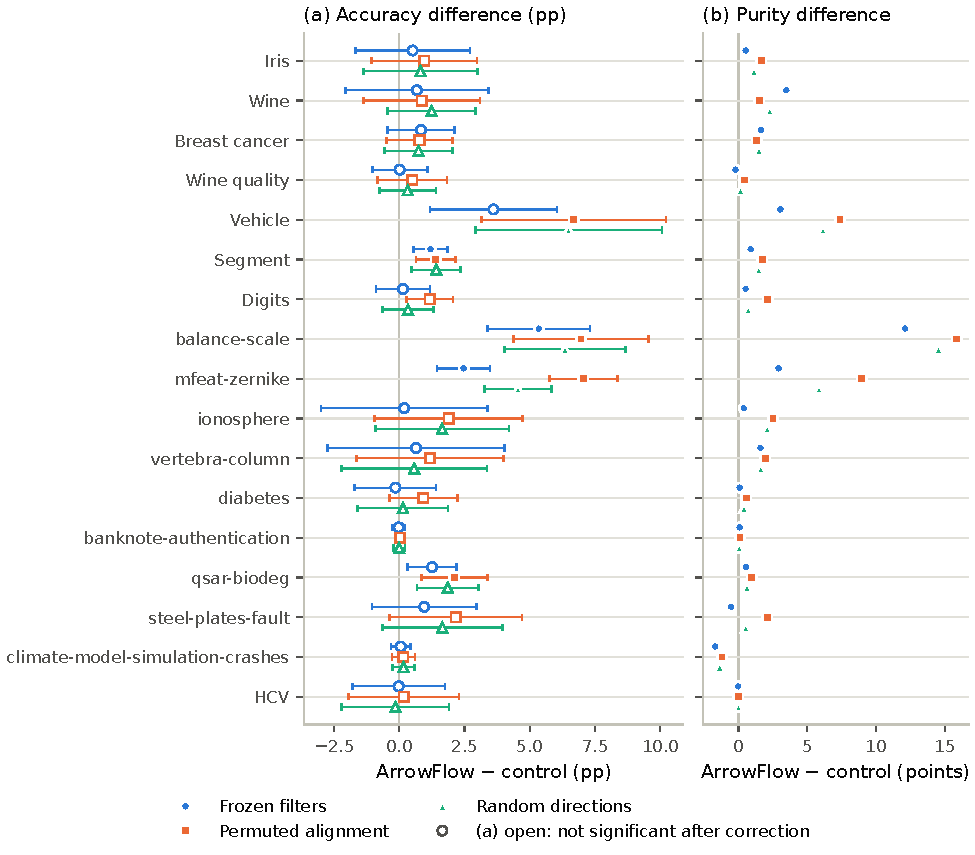
\includegraphics[width=0.92\textwidth]{figures/data/fig8_motion_forest.pdf}
\caption{\textbf{Is it the signal that helps?} (a)~ArrowFlow's accuracy minus that of each control, in percentage points, with 95\% intervals (not simultaneous); positive favors ArrowFlow. Frozen filters: the hidden filters never move. Permuted alignment: each motion reaches a filter of the same layer drawn at random, afresh in every batch. Random directions: the directions of the motions are shuffled. Both scrambled controls keep the number of motions, their sizes and their total weight. Filled marks in panel (a) remain significant after a Holm correction across the seventeen datasets within each control: 3 datasets for frozen filters, 5 for permuted alignment and 3 for random directions. The intervals are not adjusted for multiple comparisons, so an open mark's interval can exclude zero. In panel (a), ArrowFlow is more accurate than frozen filters on 14 of the 17 datasets, than permuted alignment on 17 and than random directions on 16. (b)~Neighborhood purity, how often an example's nearest training examples share its class: ArrowFlow minus each control, in percentage points, on the test rows; descriptive, with no interval and no test, so its marks carry no fill coding. ArrowFlow is purer than all three controls on 13 of the 17 datasets. In both panels, a scramble's mark to the right of the mark of frozen filters means that the scramble is less accurate than frozen filters, or in panel~(b) less pure. Tables~S28 and~S29 give these comparisons directly. HCV: hepatitis C virus.}
\label{fig:motion-forest}
\end{figure}


A scrambled signal leaves the network less accurate than no training at all. Delivering the motions to the wrong filters does so on 16 of the 17 datasets, and shuffling their directions on 14 of the 17. These counts are descriptive, but a post hoc one-sided signed-rank test across the datasets supports both ($p<0.001$; Table~S28). The neighborhoods that the readout uses degrade in the same way. We measure them by their purity, how often an example's nearest training examples share its class. On most datasets, an example's nearest training examples share its class less often after either scramble than with frozen filters (Figure~\ref{fig:motion-forest}b and Table~S29). So the motions carry information about which filter should move and in which direction. A permutation fixed for the whole of training, the analog of feedback alignment \citep{lillicrap2016random}, was not tested (Section~S3.6).

Figure~\ref{fig:motion-forest}a compares ArrowFlow itself with each control. Against frozen filters ArrowFlow is more accurate on 14 of the 17 datasets, fewer than the 16 against the untrained ArrowFlow of Section~\ref{sec:training-controls}, which chooses its own settings. The three exceptions lie within 0.2 points of zero, and the mean gain is about one point against either. The two scrambles differ in strength, so each is compared with frozen filters rather than with the other (Section~S3.6).

\subsection{What Training Does and Where It Stops}\label{sec:controlled}

The studies below look inside the trained networks and test the limits of the approach.

\paragraph{What does training teach the network?} One dataset makes this easy to see. In the balance-scale data, each example places a weight at some distance on each side of a balance. The task is to say whether the balance tips left, tips right or stays level. A level balance is rare, about one example in thirteen, and it is hard to spot, because it sits exactly on the line between the other two outcomes. Before training, ArrowFlow almost never recognizes a level balance, and neither do simpler nearest-neighbor methods on the same inputs. None of them gets more than 5 in 100 right. After training, ArrowFlow gets about half of them right. The two common outcomes are easy either way. ArrowFlow recognizes tips to either side nearly always, before training and after. So most of what training adds on this dataset comes from learning this one thin class. The support vector classifier recognizes nearly every level balance, far more often than ArrowFlow, so other methods can find this class too (Section~S3.7).

\paragraph{Do the filters move at all?} The validation checkpoint could, in principle, hand back the random starting filters. It never did. In none of the 1,785 trained views of one fitting seed did the checkpoint keep the initial filters, and in the networks with one hidden layer nearly every hidden filter ended in a new order. Ties limit what the layers can express, though. The distances from an input to many filters bunch together in a narrow band (Section~\ref{sec:theory-margin}). So two filters often sit at exactly the same distance from an input, and their IDs then decide their order. In a hidden layer of 128 filters that ranks 32 items, about four in five distances are shared with another filter, before training and after, as with random filters (Section~S3.7).

\paragraph{Does a second hidden layer help?} It did not. We refitted every split with one hidden layer of 128 filters and with two, of 64 and then 128 filters. Every other setting, including the 200 updates and the learning rate, was the one chosen for that split. On 185 of the 255 splits, that choice was made for a network with one hidden layer. With the earlier relay, one hidden layer was more accurate than two on 15 of the 17 datasets, although no difference was significant after correction. With the corrected relay, two layers were about as accurate as one, and a second layer still did not help (Section~S3.7). Over the datasets, two layers minus one averaged $-0.24$ points, with a post hoc 95\% interval from $-0.60$ to $+0.12$.

\paragraph{Does the voting rule make a difference?} Each update merges its votes by a weighted Borda count, one of the three exchangeable stages of Section~\ref{sec:arrow}. We replaced it in the hidden layers by the footrule median, the ranking with the smallest total footrule distance to the votes. Its prior weight, the weight of the filter's current order, was set once, on training data from two datasets, so that it moved the filters about as often as the Borda count there. Over all datasets it moves them less often, and per dataset the movement differs widely (Section~S3.7). The Borda count was more accurate on 13 of the 17 datasets, but significantly so only on Vehicle. This compares two voting rules and does not test Arrow's theorem (Section~S3.7).

\paragraph{Do established methods do as well?} Could an established method match ArrowFlow without any learned filters? On most datasets, yes. Take a support vector classifier with a fixed Kendall kernel \citep{jiao2015kernels,jiao2018kendall}. It compares two rankings by Kendall's $\tau$, the share of item pairs that they order alike minus the share that they order differently. Applied to rankings from ArrowFlow's own encoder, with its encoder settings chosen on its own inner folds, the classifier is more accurate than ArrowFlow on 14 of the 17 datasets. The angle property of Section~\ref{sec:theory-alphabet} suggests why. For a random view, the expected $\tau$ of two encoded rankings over the draw of the projection is $1-2\theta/\pi$, where $\theta$ is the angle between their expanded, standardized features (Section~S1.6). Up to a scale and a shift, this is the arc-cosine kernel of order zero \citep{cho2009kernel}, so the classifier acts much like a kernel machine on the features. ArrowFlow has a higher mean accuracy than nearest neighbors after a linear discriminant projection on 12 of the 17 datasets, and after a principal component projection on 11. After a learned metric (neighborhood components analysis), it has the higher mean accuracy on only 7 of the 17 (Section~S3.7).

\paragraph{Does training improve the representation itself?} ArrowFlow reads its hidden rankings with a nearest-neighbor vote. Training could improve the rankings themselves, or it could only arrange them to suit that vote. To tell the two apart, we read the untrained and the trained hidden rankings with a strong fixed readout, a support vector classifier with the same Kendall kernel. On the ten further datasets, the scope fixed in advance, the trained rankings had the higher mean accuracy on only 3, and no difference was significant. Over the ten datasets, trained minus untrained averaged $-0.10$ points, with a post hoc 95\% interval from $-0.56$ to $+0.35$. For this outcome, the protocol had fixed the following statement before the test. Training improves the nearest-neighbor neighborhoods but not the representation read by a strong fixed readout (Section~S3.7).

\subsection{Can the Ranking Signal Train the Encoder?}\label{sec:learned}

The motions have so far trained ranking filters. Here we ask whether they can also train the real-valued weights of the encoder network of Section~\ref{sec:learned-encoder}, and whether ArrowFlow gains from the trained encoder. The answer to the first is yes, and the answer to the second is a modest yes, by a rule fixed before the run (Figure~\ref{fig:learned}). Both studies below use the benchmark's test sets, but the target conversion and its settings were developed on single splits of twelve of its seventeen datasets (Section~\ref{sec:protocol}).

% Figure: the learned encoder. Rendered by render_tables.py via render_figures.encoder_forest from the run files of the
% two studies of the learned encoder; nothing numeric is typed here.
% supplement-ref supp:learned-swap=S6.4
% supplement-ref supp:learned-development=S6.2
\begin{figure}[!htbp]
\centering
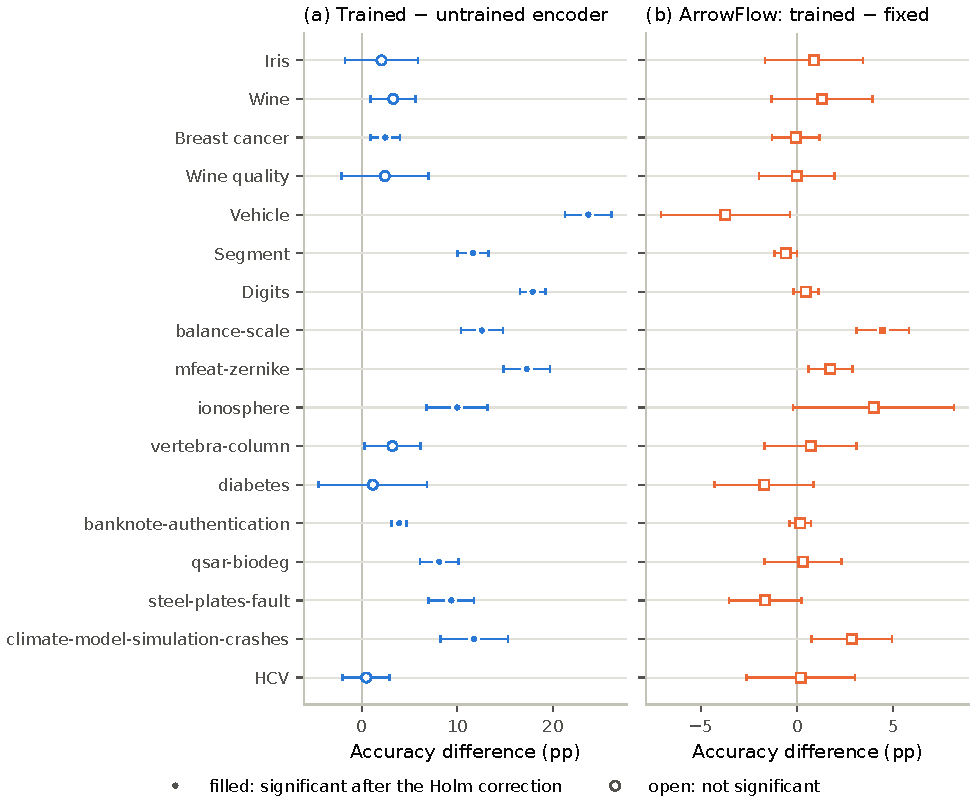
\includegraphics[width=0.92\textwidth]{figures/data/fig9_learned_encoder.pdf}
\caption{\textbf{Can the ranking signal train the encoder?} Accuracy differences, in percentage points, with 95\% intervals (not simultaneous); positive favors the trained encoder. The two panels have different scales. The intervals are not adjusted for multiple comparisons, so an open mark's interval can exclude zero. (a)~The classifier of Section~\ref{sec:learned-encoder}, an encoder network and one ranking layer of class filters, with the encoder trained by the converted motions, minus the same classifier with the encoder left at its random start. At that start, the weights of the encoder's first two layers are drawn uniformly from 0 to 1. Training lowers the mean error over the datasets from 25.5 to 17.2 percent. (b)~ArrowFlow with each view's fixed encoder replaced by the trained encoder network, minus ArrowFlow with its fixed encoder. For every split, both use the configuration that ArrowFlow's own tuning chose on the inner folds of that split's training partition. The swap also drops the polynomial expansion and the projection strategies (Section~S6.4). The mean error falls from 15.5 to 14.9 percent. Marks are circles in panel~(a) and squares in panel~(b). Filled marks remain significant after a Holm correction across the seventeen datasets: 11 in panel~(a) and 1 in panel~(b). The trained encoder has the higher mean accuracy on all 17 datasets in panel~(a) and on 11 of the 17 in panel~(b). The target conversion was developed on twelve of these datasets, all but Wine quality, banknote-authentication, qsar-biodeg, climate-model-simulation-crashes and HCV (Section~S6.2). HCV: hepatitis C virus.}
\label{fig:learned}
\end{figure}


\paragraph{Does the encoder network learn?} We tested the encoder network with one ranking layer of class filters on top, tuned on the same inner folds and scored on the same test sets (Section~S6.3). Trained by the converted motions, it was more accurate than the same network left at its random start on all 17 datasets, significantly so on 11 (Figure~\ref{fig:learned}a). So a discrete ranking signal trains continuous weights without differentiating the sort, as other methods that keep the ranking step exact also do (Section~\ref{sec:related}). The untrained encoder is a weak reference, though. Its first two layers start with weights drawn uniformly from 0 to 1, and its mean error is 25.5 percent, against 17.2 percent after training. The largest gain, 23.7 points on Vehicle, started from an error of 48.7 percent.

Two more contrasts were fixed before the run. Read by its class filters, the trained classifier still trails the tuned MLP. It is ahead on 3 datasets, significantly on none, and significantly behind on 4. Read instead by a nearest-neighbor vote, a single trained encoder with no hidden ranking layer comes close to ArrowFlow, with a mean error of 15.6 against 15.5 percent (Section~S6.3).

\paragraph{Does ArrowFlow gain from it?} We then rebuilt ArrowFlow for every split, with the configuration that ArrowFlow's own tuning chose on the inner folds of that split's training partition. In each view, an encoder network trained on the view's training rows replaced the fixed encoder (Section~S6.4). This also removed the polynomial expansion and the three projection strategies. The views then differed only by their seeds, and no view used linear discriminant coordinates. With the fixed encoder, the rebuild reproduced the stored predictions exactly on the four test sets we checked, at all three fitting seeds (12 fits; Section~S6.4).

With the trained encoder network, ArrowFlow had the higher mean accuracy on 11 of the 17 datasets, significantly on balance-scale, and was significantly less accurate on none (Figure~\ref{fig:learned}b). Its mean error over the datasets fell from 15.5 to 14.9 percent. The rule fixed before the run has two conditions: a higher mean accuracy, and more datasets significantly higher than significantly lower. Both hold, so the rule reads that the trained encoder improves ArrowFlow. A single dataset, balance-scale, meets the second condition, and the conversion was developed partly on it. Across the datasets the gain is not established (post hoc one-sided signed-rank test, $p=0.095$). Left untrained, the same network made ArrowFlow less accurate than the fixed encoder did on 16 of the 17 datasets. So the gain comes from training. Swapping in the network alone makes ArrowFlow worse.

\paragraph{How far does it go?} The trained encoder made ArrowFlow less accurate on 6 of the 17 datasets, by up to 3.7 points on Vehicle, although none of these losses was significant. Every configuration had been tuned for the fixed encoder, which favors the fixed encoder in this comparison. With the trained encoder, ArrowFlow's mean error of 14.9 percent is close to the tuned MLP's 14.6. On balance-scale its error of 1.6 percent is the lowest of all the tuned models. But it still trails the best tuned classical model on 15 of the 17 datasets (Section~S6.4). These comparisons are descriptive, and on balance-scale the lead over the MLP is not significant. The MLP reached its iteration cap before convergence on 331 of its 765 outer fits (Section~S3.2). Against the single trained encoder read by a nearest-neighbor vote, ArrowFlow with the trained encoder is ahead on 15 of the 17 datasets, by 0.67 points on average, and significantly on none (Section~S6.4).

% Supplement subsections typed below as "Section~S<n>.<m>"; build.sh checks each number against the built supplement.
% supplement-ref supp:sorting=S3.4
% supplement-ref supp:iia=S1.1
% supplement-ref supp:learned-development=S6.2
% supplement-ref supp:motion=S3.6
% supplement-ref supp:controlled=S3.7
\section{Discussion}\label{sec:discussion}

This paper set out to show that a network can compute with rankings and learn by counting votes. The experiments support that claim and one more. A learning rule that computes no derivative trains ranking layers, and the signal it sends down carries information. Motions of the same kind can also train a real-valued encoder network. But ArrowFlow trails the best tuned classical model on all seventeen small tabular datasets, and training its ranking layers adds only a modest gain. So the contribution is a construction and a learning rule inside permutation space, and the paper makes no accuracy argument.

\paragraph{What the training signal carries.}
The central finding is about the signal. Training helps because of the particular signal that the output layer returns, and matched controls separate that signal from mere movement of the filters (Section~\ref{sec:motion-controls}). If the update were only a useful disturbance, a scramble of the same size would cost nothing. Instead, a scrambled signal is worse than freezing the filters altogether, as a post hoc test across the datasets supports. And on most datasets it leaves an example's nearest neighbors less likely to share its class. Both parts of the signal carry information: which filter a motion reaches, and which way it points. Permuted alignment drew a new random assignment of motions to filters in every batch, and a fixed wrong assignment was not tested (Section~S3.6).

\paragraph{What training adds.}
Training adds a modest gain, and an untrained network already does well. With the same readout, the untrained ArrowFlow comes within one percentage point of ArrowFlow on 12 of the 17 datasets. It is a permutation analog of random-weight models, which fix random hidden units and train only a readout \citep{pao1994learning,huang2006extreme}. It is also an analog of random features for kernel machines \citep{rahimi2007random}. In the cited studies, such models generalized well on the benchmarks tested \citep{huang2006extreme} and matched or outperformed kernel machines there \citep{huang2012extreme,rahimi2007random}. The untrained ArrowFlow differs from them in two ways. Its units are permutations, and its readout is a nearest-neighbor vote rather than a least-squares linear map. Moreover, three of its seven views use the class labels, through a linear discriminant projection.

Read by a strong fixed readout, a Kendall-kernel classifier, the trained hidden rankings are no better than the untrained ones (Section~\ref{sec:controlled}). So training improves the neighborhoods that the nearest-neighbor readout uses. It does not improve the representation that a strong readout sees. Where the gain is large, it can sit in one place. On balance-scale, most of it comes from the rare class of level balances, which the support vector classifier recognizes far more often (Section~\ref{sec:controlled}). This locates the gain. It does not show that the network discovered the physical rule of the balance.

\paragraph{What the trained encoder adds.}
Motions can train more than ranking filters. Turned into target scores, they train the weights of an encoder network across a sort that is never differentiated. As a classifier, the trained encoder is more accurate than the same network untrained on every dataset, significantly on 11 (Section~\ref{sec:learned}). The step is target propagation applied at a discrete interface \citep{bengio2014auto,lee2015difference,friesen2018combinatorial}. It does not relax the sort \citep{grover2019neuralsort,blondel2020fast}, and it does not copy a gradient across it \citep{bengio2013estimating}. Still, with evenly spaced scores the step points the same way as a straight-through estimate for the same targets. The conversion multiplies each coordinate's requested change of position by the gap between neighboring scores. A straight-through estimate that treats position as a linear function of score divides by that gap instead. Other methods also train through an exact discrete step (Section~\ref{sec:related}), among them blackbox differentiation \citep{vlastelica2020differentiation,rolinek2020optimizing} and perturbed optimizers \citep{berthet2020perturbed}. This paper does not compare the conversion with them. Inside ArrowFlow the gain is modest and uneven. One dataset improves significantly and none worsens significantly, but six lose some accuracy. The comparison favors the fixed encoder, because every configuration was tuned for it. The encoder network is one small architecture, and the conversion and its settings were developed on single splits of twelve of the seventeen datasets before these runs (Section~S6.2). The main method therefore keeps the fixed encoder. How well networks that mix ranking layers with ordinary layers can do when both are tuned together is still an open question.

\paragraph{What the Arrow lens delivers.}
The lens does two things. First, it locates context dependence. When the current order counts as a voter, no rule can avoid it. Consider any update rule in the setting of Proposition~\ref{prop:borda-iia} that meets two mild conditions. It never reverses a pair on which the current order and all votes agree, and it neither freezes the filter nor always copies one vote. Every such rule is context dependent. Under the weight condition of Proposition~\ref{prop:borda-iia}, the weighted Borda count that updates a filter violates independence of irrelevant alternatives when the filter's current order counts as a voter. An actual update holds that order fixed. In ArrowFlow's layers it is then not Pareto efficient, so Arrow's theorem does not cover it. A direct construction still shows a violation whenever its votes can move the filter (Section~S1.1). A version of Arrow's theorem without Pareto efficiency, Wilson's theorem, implies the violation once the votes of a batch outweigh the current order \citep{wilson1972pareto}. So a filter's order of two items can depend on a third. The forward pass has no such dependence within a layer.

Second, the voting reading names three stages whose rules can be exchanged, although Arrow's theorem speaks only to the update. The experiments exchanged all three, the view stage only with the prototype readout. The nearest-neighbor readout was more accurate than the prototype readout. Against a footrule median inside ArrowFlow's own layers, the Borda count had the higher mean accuracy on 13 of the 17 datasets, significantly on one. Post hoc, the median learned little. On some datasets it barely moved the filters. On most others it moved them but ended within 0.2 points of untrained filters (Section~S3.7). Across views, with the prototype readout, Borda and majority votes differ by at most $0.6$ percentage points (Section~S4). The lens predicted none of these outcomes. We claim no expressive power from the axiom violation, and the voting-rule study is not a test of Arrow's theorem.

\paragraph{Boundaries.}
A second hidden layer did not improve accuracy at a matched configuration, with the earlier relay or with the corrected one. The rule passes supervision through several ranking layers, but the second layer brought no measured benefit. No experiment showed that the relayed signal improves the first layer. On the seven benchmark datasets, sorting the projected scores made no detectable difference to a nearest-neighbor readout, so there the ranking itself cannot be credited with any gain in accuracy. On the ten further datasets, where the comparison is descriptive, sorting raised the error on six, by up to 2.5 points (Section~S3.4).

\paragraph{Limitations.}
Seventeen small tabular datasets are a narrow basis. The largest training partition has 1,848 rows (Segment). Fifteen test sets give wide intervals, and a difference that is not significant does not show that two models are equal. The candidate grid was small and anchored on default settings. A wider search inside the training data could move Table~\ref{tab:main} in either direction. Settings were chosen by accuracy, and the readout does not weight classes. So a rare class can be neglected (Section~\ref{sec:main-benchmark}). Each study's own limits, such as single fitting seeds and unmatched architectures, are stated with its details in Sections~S3 and~S4.

\section{Conclusion}\label{sec:conclusion}

We asked whether a network can compute with rankings and learn by counting votes, with no derivative computed. Each ranking layer orders its learned permutations by footrule distance to its input, and votes reorder the filters. The motions returned by the output layer's votes train the last hidden layer, and every hidden layer above the first relays signed motions to the one below. Most experiments used an earlier version of this relay, which differs only in networks with two hidden layers (Section~\ref{sec:training}). A nearest-neighbor vote on the last hidden ranking predicts the class. Every filter update is an election decided by a weighted Borda count in which the filter's current order also votes. Under a mild weight condition this rule violates independence of irrelevant alternatives by Arrow's theorem (Section~\ref{sec:arrow}). An update that holds the current order fixed violates it too, by a direct construction, whenever its votes can move the filter.

Matched controls and a post hoc test across the datasets indicate that the returned motions carry information. Scrambling which filter a motion reaches, or which way it points, leaves the network less accurate than never moving the filters at all (Section~\ref{sec:motion-controls}). Motions of the same kind also train an ordinary neural network. Turned into target scores, they train an encoder network across a sort that is never differentiated. Swapped into ArrowFlow for its fixed encoder, the trained encoder raised the mean accuracy on 11 of the 17 datasets, significantly on one, and lowered it significantly on none (Section~\ref{sec:learned}).

The limits are just as clear. With every configuration chosen inside the training data, ArrowFlow trails the best tuned classical model on all seventeen tabular datasets (Table~\ref{tab:main}). Its average rank, fourth of six, lies between random forest and gradient boosting; on the ten further datasets alone it is fifth. So this paper offers a learning rule inside permutation space, and no gain in accuracy (Section~\ref{sec:controlled}). A second hidden layer did not improve accuracy.

Whether deeper hierarchies and larger datasets gain more from training remains open. How far networks that mix ranking layers with ordinary layers can go is still open.


% ============================================================================
% BACK MATTER (MDPI order; the Data Availability Statement and the Acknowledgments keep their approved wording)
% ============================================================================
\section*{Supplementary Materials}
% Supplement numbers typed below; build.sh checks each against the built supplement (the first table and the
% two figures are declared under the Data Availability Statement).
% supplement-ref tab:s-learned-swap-controls=S75
The supplementary material is a separate document with six sections: the proofs (Section~S1), the method details, worked example and protocol (Section~S2), the complete results (Section~S3), the ablations (Section~S4), the reproducibility records (Section~S5) and the learned encoder (Section~S6). It contains Tables~S1 to~S75 and Figures~S1 to~S5.

\section*{Author Contributions}
Conceptualization, methodology, software, validation, formal analysis, investigation, data curation, writing (original draft preparation, review and editing) and visualization: O.Y. The author has read and agreed to the published version of the manuscript.

\section*{Funding}
This research received no external funding.

\section*{Institutional Review Board Statement}
Not applicable. The study analyzes only public, de-identified datasets.

\section*{Informed Consent Statement}
Not applicable.

\section*{Data Availability Statement}
% Supplement numbers typed below; build.sh checks each against the built supplement.
% supplement-ref supp:datasets=S5.2
% supplement-ref supp:selection=S3.1
% supplement-ref supp:worked-example=S2.2
% supplement-ref tab:settings=S1
% supplement-ref tab:settings-readout=S2
% supplement-ref tab:study-map=S4
% supplement-ref fig:s-weight-regimes=S1
% supplement-ref fig:s-angle=S2
% supplement-ref fig:s-nested-cv=S3
% supplement-ref fig:learning-controls=S4
% supplement-ref fig:learning-curves=S5

The datasets are public. The seven benchmark datasets originate from the University of California, Irvine (UCI) Machine Learning Repository; we used the copies distributed with scikit-learn for Iris, Wine, Breast cancer and Digits and OpenML copies for Wine quality, Vehicle and Segment. The ten further datasets come from OpenML. Section~S5.2 gives the source and content hash of every copy and the identifier of every OpenML copy, which names one fixed version; the protocols of the further datasets also pin their versions and file checksums (Section~S3.1). The reference list cites each dataset.

The implementation, the harness that ran every experiment and the frozen protocol files are available at \url{https://github.com/yilmazozgur/arrowflow}, release \mbox{v2.0.0-make}. Section~S5 lists every protocol file with its identifier, freeze time and code revision, and gives the environment and the commands that reproduce each family.

Every results table of this paper and its supplement, Figures~\ref{fig:motion-forest} and~\ref{fig:learned} and Figures~S4 and~S5 are rendered by a script from the recorded run directories, and the script checks the numbers and counts that the text quotes from those runs. Tables~\ref{tab:notation} and~\ref{tab:overview}, Tables~S1, S2 and~S4, Figures~\ref{fig:pipeline} to~\ref{fig:cones}, Figures~S1 to~S3 and the worked example of Section~S2.2 are written by hand; the test suite checks the worked example. The run directories and the rendering script are available from the author on request.

\section*{Acknowledgments}
During the preparation of this work the author used Claude Opus 5, Claude Opus 5.5, Claude Fable 5 and Claude Fable 5.1 (Anthropic), and GPT 5.6 Sol and GPT 6 Astra (OpenAI) for software development, running and analysing the experiments, and editing the manuscript. The author reviewed all output and takes full responsibility for the content of the publication.

\section*{Conflicts of Interest}
The author declares no conflicts of interest.

% ============================================================================
% REFERENCES
% ============================================================================
\bibliographystyle{plainnat}
\bibliography{references_v3}

\end{document}
